% Options for packages loaded elsewhere
\PassOptionsToPackage{unicode}{hyperref}
\PassOptionsToPackage{hyphens}{url}
\PassOptionsToPackage{dvipsnames,svgnames,x11names}{xcolor}
%
\documentclass[
]{article}

\usepackage{amsmath,amssymb}
\usepackage{iftex}
\ifPDFTeX
  \usepackage[T1]{fontenc}
  \usepackage[utf8]{inputenc}
  \usepackage{textcomp} % provide euro and other symbols
\else % if luatex or xetex
  \usepackage{unicode-math}
  \defaultfontfeatures{Scale=MatchLowercase}
  \defaultfontfeatures[\rmfamily]{Ligatures=TeX,Scale=1}
\fi
\usepackage{lmodern}
\ifPDFTeX\else  
    % xetex/luatex font selection
\fi
% Use upquote if available, for straight quotes in verbatim environments
\IfFileExists{upquote.sty}{\usepackage{upquote}}{}
\IfFileExists{microtype.sty}{% use microtype if available
  \usepackage[]{microtype}
  \UseMicrotypeSet[protrusion]{basicmath} % disable protrusion for tt fonts
}{}
\makeatletter
\@ifundefined{KOMAClassName}{% if non-KOMA class
  \IfFileExists{parskip.sty}{%
    \usepackage{parskip}
  }{% else
    \setlength{\parindent}{0pt}
    \setlength{\parskip}{6pt plus 2pt minus 1pt}}
}{% if KOMA class
  \KOMAoptions{parskip=half}}
\makeatother
\usepackage{xcolor}
\usepackage[lmargin=1in,rmargin=1in,tmargin=1in,bmargin=1in]{geometry}
\setlength{\emergencystretch}{3em} % prevent overfull lines
\setcounter{secnumdepth}{5}
% Make \paragraph and \subparagraph free-standing
\makeatletter
\ifx\paragraph\undefined\else
  \let\oldparagraph\paragraph
  \renewcommand{\paragraph}{
    \@ifstar
      \xxxParagraphStar
      \xxxParagraphNoStar
  }
  \newcommand{\xxxParagraphStar}[1]{\oldparagraph*{#1}\mbox{}}
  \newcommand{\xxxParagraphNoStar}[1]{\oldparagraph{#1}\mbox{}}
\fi
\ifx\subparagraph\undefined\else
  \let\oldsubparagraph\subparagraph
  \renewcommand{\subparagraph}{
    \@ifstar
      \xxxSubParagraphStar
      \xxxSubParagraphNoStar
  }
  \newcommand{\xxxSubParagraphStar}[1]{\oldsubparagraph*{#1}\mbox{}}
  \newcommand{\xxxSubParagraphNoStar}[1]{\oldsubparagraph{#1}\mbox{}}
\fi
\makeatother

\usepackage{color}
\usepackage{fancyvrb}
\newcommand{\VerbBar}{|}
\newcommand{\VERB}{\Verb[commandchars=\\\{\}]}
\DefineVerbatimEnvironment{Highlighting}{Verbatim}{commandchars=\\\{\}}
% Add ',fontsize=\small' for more characters per line
\usepackage{framed}
\definecolor{shadecolor}{RGB}{241,243,245}
\newenvironment{Shaded}{\begin{snugshade}}{\end{snugshade}}
\newcommand{\AlertTok}[1]{\textcolor[rgb]{0.68,0.00,0.00}{#1}}
\newcommand{\AnnotationTok}[1]{\textcolor[rgb]{0.37,0.37,0.37}{#1}}
\newcommand{\AttributeTok}[1]{\textcolor[rgb]{0.40,0.45,0.13}{#1}}
\newcommand{\BaseNTok}[1]{\textcolor[rgb]{0.68,0.00,0.00}{#1}}
\newcommand{\BuiltInTok}[1]{\textcolor[rgb]{0.00,0.23,0.31}{#1}}
\newcommand{\CharTok}[1]{\textcolor[rgb]{0.13,0.47,0.30}{#1}}
\newcommand{\CommentTok}[1]{\textcolor[rgb]{0.37,0.37,0.37}{#1}}
\newcommand{\CommentVarTok}[1]{\textcolor[rgb]{0.37,0.37,0.37}{\textit{#1}}}
\newcommand{\ConstantTok}[1]{\textcolor[rgb]{0.56,0.35,0.01}{#1}}
\newcommand{\ControlFlowTok}[1]{\textcolor[rgb]{0.00,0.23,0.31}{\textbf{#1}}}
\newcommand{\DataTypeTok}[1]{\textcolor[rgb]{0.68,0.00,0.00}{#1}}
\newcommand{\DecValTok}[1]{\textcolor[rgb]{0.68,0.00,0.00}{#1}}
\newcommand{\DocumentationTok}[1]{\textcolor[rgb]{0.37,0.37,0.37}{\textit{#1}}}
\newcommand{\ErrorTok}[1]{\textcolor[rgb]{0.68,0.00,0.00}{#1}}
\newcommand{\ExtensionTok}[1]{\textcolor[rgb]{0.00,0.23,0.31}{#1}}
\newcommand{\FloatTok}[1]{\textcolor[rgb]{0.68,0.00,0.00}{#1}}
\newcommand{\FunctionTok}[1]{\textcolor[rgb]{0.28,0.35,0.67}{#1}}
\newcommand{\ImportTok}[1]{\textcolor[rgb]{0.00,0.46,0.62}{#1}}
\newcommand{\InformationTok}[1]{\textcolor[rgb]{0.37,0.37,0.37}{#1}}
\newcommand{\KeywordTok}[1]{\textcolor[rgb]{0.00,0.23,0.31}{\textbf{#1}}}
\newcommand{\NormalTok}[1]{\textcolor[rgb]{0.00,0.23,0.31}{#1}}
\newcommand{\OperatorTok}[1]{\textcolor[rgb]{0.37,0.37,0.37}{#1}}
\newcommand{\OtherTok}[1]{\textcolor[rgb]{0.00,0.23,0.31}{#1}}
\newcommand{\PreprocessorTok}[1]{\textcolor[rgb]{0.68,0.00,0.00}{#1}}
\newcommand{\RegionMarkerTok}[1]{\textcolor[rgb]{0.00,0.23,0.31}{#1}}
\newcommand{\SpecialCharTok}[1]{\textcolor[rgb]{0.37,0.37,0.37}{#1}}
\newcommand{\SpecialStringTok}[1]{\textcolor[rgb]{0.13,0.47,0.30}{#1}}
\newcommand{\StringTok}[1]{\textcolor[rgb]{0.13,0.47,0.30}{#1}}
\newcommand{\VariableTok}[1]{\textcolor[rgb]{0.07,0.07,0.07}{#1}}
\newcommand{\VerbatimStringTok}[1]{\textcolor[rgb]{0.13,0.47,0.30}{#1}}
\newcommand{\WarningTok}[1]{\textcolor[rgb]{0.37,0.37,0.37}{\textit{#1}}}

\providecommand{\tightlist}{%
  \setlength{\itemsep}{0pt}\setlength{\parskip}{0pt}}\usepackage{longtable,booktabs,array}
\usepackage{calc} % for calculating minipage widths
% Correct order of tables after \paragraph or \subparagraph
\usepackage{etoolbox}
\makeatletter
\patchcmd\longtable{\par}{\if@noskipsec\mbox{}\fi\par}{}{}
\makeatother
% Allow footnotes in longtable head/foot
\IfFileExists{footnotehyper.sty}{\usepackage{footnotehyper}}{\usepackage{footnote}}
\makesavenoteenv{longtable}
\usepackage{graphicx}
\makeatletter
\newsavebox\pandoc@box
\newcommand*\pandocbounded[1]{% scales image to fit in text height/width
  \sbox\pandoc@box{#1}%
  \Gscale@div\@tempa{\textheight}{\dimexpr\ht\pandoc@box+\dp\pandoc@box\relax}%
  \Gscale@div\@tempb{\linewidth}{\wd\pandoc@box}%
  \ifdim\@tempb\p@<\@tempa\p@\let\@tempa\@tempb\fi% select the smaller of both
  \ifdim\@tempa\p@<\p@\scalebox{\@tempa}{\usebox\pandoc@box}%
  \else\usebox{\pandoc@box}%
  \fi%
}
% Set default figure placement to htbp
\def\fps@figure{htbp}
\makeatother
% definitions for citeproc citations
\NewDocumentCommand\citeproctext{}{}
\NewDocumentCommand\citeproc{mm}{%
  \begingroup\def\citeproctext{#2}\cite{#1}\endgroup}
\makeatletter
 % allow citations to break across lines
 \let\@cite@ofmt\@firstofone
 % avoid brackets around text for \cite:
 \def\@biblabel#1{}
 \def\@cite#1#2{{#1\if@tempswa , #2\fi}}
\makeatother
\newlength{\cslhangindent}
\setlength{\cslhangindent}{1.5em}
\newlength{\csllabelwidth}
\setlength{\csllabelwidth}{3em}
\newenvironment{CSLReferences}[2] % #1 hanging-indent, #2 entry-spacing
 {\begin{list}{}{%
  \setlength{\itemindent}{0pt}
  \setlength{\leftmargin}{0pt}
  \setlength{\parsep}{0pt}
  % turn on hanging indent if param 1 is 1
  \ifodd #1
   \setlength{\leftmargin}{\cslhangindent}
   \setlength{\itemindent}{-1\cslhangindent}
  \fi
  % set entry spacing
  \setlength{\itemsep}{#2\baselineskip}}}
 {\end{list}}
\usepackage{calc}
\newcommand{\CSLBlock}[1]{\hfill\break\parbox[t]{\linewidth}{\strut\ignorespaces#1\strut}}
\newcommand{\CSLLeftMargin}[1]{\parbox[t]{\csllabelwidth}{\strut#1\strut}}
\newcommand{\CSLRightInline}[1]{\parbox[t]{\linewidth - \csllabelwidth}{\strut#1\strut}}
\newcommand{\CSLIndent}[1]{\hspace{\cslhangindent}#1}

\usepackage{draftwatermark}
\DraftwatermarkOptions{%
  text={INPROGRESS},
  color={[rgb]{1,0.6,0.6}}, % light red
  angle=45,
  scale=.5
}
\makeatletter
\@ifpackageloaded{tcolorbox}{}{\usepackage[skins,breakable]{tcolorbox}}
\@ifpackageloaded{fontawesome5}{}{\usepackage{fontawesome5}}
\definecolor{quarto-callout-color}{HTML}{909090}
\definecolor{quarto-callout-note-color}{HTML}{0758E5}
\definecolor{quarto-callout-important-color}{HTML}{CC1914}
\definecolor{quarto-callout-warning-color}{HTML}{EB9113}
\definecolor{quarto-callout-tip-color}{HTML}{00A047}
\definecolor{quarto-callout-caution-color}{HTML}{FC5300}
\definecolor{quarto-callout-color-frame}{HTML}{acacac}
\definecolor{quarto-callout-note-color-frame}{HTML}{4582ec}
\definecolor{quarto-callout-important-color-frame}{HTML}{d9534f}
\definecolor{quarto-callout-warning-color-frame}{HTML}{f0ad4e}
\definecolor{quarto-callout-tip-color-frame}{HTML}{02b875}
\definecolor{quarto-callout-caution-color-frame}{HTML}{fd7e14}
\makeatother
\makeatletter
\@ifpackageloaded{caption}{}{\usepackage{caption}}
\AtBeginDocument{%
\ifdefined\contentsname
  \renewcommand*\contentsname{Table of contents}
\else
  \newcommand\contentsname{Table of contents}
\fi
\ifdefined\listfigurename
  \renewcommand*\listfigurename{List of Figures}
\else
  \newcommand\listfigurename{List of Figures}
\fi
\ifdefined\listtablename
  \renewcommand*\listtablename{List of Tables}
\else
  \newcommand\listtablename{List of Tables}
\fi
\ifdefined\figurename
  \renewcommand*\figurename{Figure}
\else
  \newcommand\figurename{Figure}
\fi
\ifdefined\tablename
  \renewcommand*\tablename{Table}
\else
  \newcommand\tablename{Table}
\fi
}
\@ifpackageloaded{float}{}{\usepackage{float}}
\floatstyle{ruled}
\@ifundefined{c@chapter}{\newfloat{codelisting}{h}{lop}}{\newfloat{codelisting}{h}{lop}[chapter]}
\floatname{codelisting}{Listing}
\newcommand*\listoflistings{\listof{codelisting}{List of Listings}}
\makeatother
\makeatletter
\makeatother
\makeatletter
\@ifpackageloaded{caption}{}{\usepackage{caption}}
\@ifpackageloaded{subcaption}{}{\usepackage{subcaption}}
\makeatother

\usepackage{bookmark}

\IfFileExists{xurl.sty}{\usepackage{xurl}}{} % add URL line breaks if available
\urlstyle{same} % disable monospaced font for URLs
\hypersetup{
  pdftitle={Applied Reproducible Data Science Processes},
  pdfauthor={Adam Ross Nelson JD PhD},
  pdfkeywords={reproducible research, data science methods, public
policy, Wisconsin lakes, Python, Quarto},
  colorlinks=true,
  linkcolor={blue},
  filecolor={Maroon},
  citecolor={Blue},
  urlcolor={Blue},
  pdfcreator={LaTeX via pandoc}}


\title{Applied Reproducible Data Science Processes}
\usepackage{etoolbox}
\makeatletter
\providecommand{\subtitle}[1]{% add subtitle to \maketitle
  \apptocmd{\@title}{\par {\large #1 \par}}{}{}
}
\makeatother
\subtitle{A demonstration using data from Wisconsin lakes}
\author{Adam Ross Nelson JD PhD}
\date{2025-01-01}

\begin{document}
\maketitle
\begin{abstract}
This paper demonstrates the practical application of data science
methods through a case study of Wisconsin lakes, addressing a
fundamental question in the field: how do data scientists provide value
to organizations? Using a comprehensive dataset of 16,711 lakes from the
Wisconsin Department of Natural Resources, we present a reproducible
workflow that supports policy makers in their oversight of public
accommodations. The study serves multiple audiences---organizational
leaders, academic researchers, industry professionals, and students---by
illustrating how data science methods can generate actionable insights
through reproducible approaches. We employ Python-based analysis tools
and modern reproducible research practices, making all code, data, and
methods openly available. This work not only provides practical insights
for lake management but also serves as an educational template for
understanding the data science process, from initial data exploration to
final recommendations. The paper demonstrates how data scientists can
bridge the gap between raw data and policy decisions, while maintaining
transparency and reproducibility throughout the analytical process.
\end{abstract}

\renewcommand*\contentsname{Table of contents}
{
\hypersetup{linkcolor=}
\setcounter{tocdepth}{3}
\tableofcontents
}

INPROGRESS

\begin{Shaded}
\begin{Highlighting}[]
\CommentTok{\# Import Pandas, Seaborn, and related}
\ImportTok{import}\NormalTok{ pandas }\ImportTok{as}\NormalTok{ pd}
\ImportTok{import}\NormalTok{ numpy }\ImportTok{as}\NormalTok{ np}
\ImportTok{import}\NormalTok{ seaborn }\ImportTok{as}\NormalTok{ sns}
\ImportTok{import}\NormalTok{ matplotlib.pyplot }\ImportTok{as}\NormalTok{ plt}
\ImportTok{import}\NormalTok{ geopandas }\ImportTok{as}\NormalTok{ gpd}
\ImportTok{import}\NormalTok{ requests}

\ImportTok{import}\NormalTok{ matplotlib.pyplot }\ImportTok{as}\NormalTok{ plt}
\ImportTok{import}\NormalTok{ matplotlib.image }\ImportTok{as}\NormalTok{ mpimg}

\ImportTok{from}\NormalTok{ scipy.stats }\ImportTok{import}\NormalTok{ chi2\_contingency}

\ImportTok{from}\NormalTok{ IPython.display }\ImportTok{import}\NormalTok{ Markdown, display}

\ImportTok{from}\NormalTok{ sklearn.preprocessing }\ImportTok{import}\NormalTok{ StandardScaler}
\ImportTok{from}\NormalTok{ sklearn.preprocessing }\ImportTok{import}\NormalTok{ OneHotEncoder}
\ImportTok{from}\NormalTok{ sklearn.model\_selection }\ImportTok{import}\NormalTok{ train\_test\_split}
\ImportTok{from}\NormalTok{ sklearn.neighbors }\ImportTok{import}\NormalTok{ KNeighborsClassifier}

\CommentTok{\# Set Seaborn context}
\NormalTok{sns.set\_context(}\StringTok{\textquotesingle{}paper\textquotesingle{}}\NormalTok{)}

\CommentTok{\# Preliminary data inspections}
\NormalTok{df0 }\OperatorTok{=}\NormalTok{ pd.read\_csv(}\StringTok{\textquotesingle{}Lakes\_Original.csv\textquotesingle{}}\NormalTok{)}
\ControlFlowTok{with} \BuiltInTok{open}\NormalTok{(}\StringTok{\textquotesingle{}\_variables.yml\textquotesingle{}}\NormalTok{, }\StringTok{\textquotesingle{}a\textquotesingle{}}\NormalTok{) }\ImportTok{as}\NormalTok{ f:}
    \CommentTok{\# Write number of observations for later reference}
\NormalTok{    f.write(}\SpecialStringTok{f\textquotesingle{}number\_of\_lakes: }\SpecialCharTok{\{}\NormalTok{df0}\SpecialCharTok{.}\NormalTok{shape[}\DecValTok{0}\NormalTok{]}\SpecialCharTok{\}}\CharTok{\textbackslash{}n}\SpecialStringTok{\textquotesingle{}}\NormalTok{)}
    \CommentTok{\# Write number of records with 0°, 0° Latitude and Longitude}
\NormalTok{    f.write(}\SpecialStringTok{f\textquotesingle{}zero\_coords\_count: }\SpecialCharTok{\{}\NormalTok{df0[df0[}\StringTok{"Latitude"}\NormalTok{] }\OperatorTok{==} \DecValTok{0}\NormalTok{]}\SpecialCharTok{.}\NormalTok{shape[}\DecValTok{0}\NormalTok{]}\SpecialCharTok{\}}\CharTok{\textbackslash{}n}\SpecialStringTok{\textquotesingle{}}\NormalTok{)}
\end{Highlighting}
\end{Shaded}

\begin{tcolorbox}[enhanced jigsaw, coltitle=black, toprule=.15mm, arc=.35mm, bottomtitle=1mm, opacityback=0, leftrule=.75mm, left=2mm, colframe=quarto-callout-note-color-frame, toptitle=1mm, titlerule=0mm, breakable, colbacktitle=quarto-callout-note-color!10!white, colback=white, bottomrule=.15mm, title=\textcolor{quarto-callout-note-color}{\faInfo}\hspace{0.5em}{Note}, rightrule=.15mm, opacitybacktitle=0.6]

As provided by the Wisconsin Department of Natural Resrouces the data
for this project includes 14 columns of information from 16711 lakes.
(Wisconsin Department of Natural Resources 2024).

\end{tcolorbox}

\section{Introduction}\label{introduction}

A common question faced by organizational executive leadership (the
c-suite), academic researchers, industry professionals, students, and
others regarding data science methods or models is what do these methods
and models accomplish. Closely related is what does a data scientist do?
Or, how does a data scientist provide value to an organization? These
are important questions becuase as Raschka and Mirjalili (2019) point
out large companies ``heavily invest in machine learning research
applicaionts for \emph{good reason}'' (p.~xiii) (emphasis added). This
paper presents a novel response to those questions.

I write this paper for at least four audiences who all have a common
interest.

\begin{itemize}
\tightlist
\item
  First for organizational leaders who may not seek to employ these
  methods on their own but who have an interest in developing or
  acquiring talent who can employ these methods.
\item
  Second, for academic researchers who are situated in universities,
  think takes, or research institues and who are often funded by private
  or government research grants.
\item
  Third, for industry professionals who may work in for-profit,
  not-for-profit, or governmental organizations.
\item
  And fourth for students, at any level of study but who may be newer to
  the exploration of data science.
\end{itemize}

These audiences share a common interest in understanding the practical
utility of data science methods and models. Each of thease audiences
have a need to understand how data science can offer highly reproducible
approaches, results, insights, utility, and other forms of valuable
output. To assist in meeting these common objectives I also distribute
with this paper its raw markdown, Python code, Jupyter notebooks, and
data sources.

This paper presents an example of work that might have been performed by
a data scientist who is working to support policy makers as they oversee
the maintenance of public accommodations on lakes located across the
State of Wisconsin. This paper's example does not put a model into
production because the contexts do not demand a model in production.

The guiding analytical question and goal for this paper is to use data
science as a means to explore which lakes have public services such as a
park, beach, or boat landing but perhaps should not. Conversely also to
explore which lakes should have public services such as a park, breach,
or boat landing but perhaps do not.

Those that have a service but perhaps should not I will describe as
overserviced while those that do not have service but perhaps should I
will describe as underserviced.

\section{Literature Review}\label{literature-review}

This literature review serves to provide an overview of three important
contexts that inform this paper's analytical approach including the
policy context, the environmental/limnological/geologic context, and the
practice of data science.

\subsection{Policy Context}\label{policy-context}

The goal of this project is to inform multiple autorities and decision
makers as they work in collaboration to make and implement public
policy. This context, where also multiple sources of authority conflict
in their interests, may benefit from an analysis that identifies
underserviced or overserviced lakes.

The management of Wisconsin's lakes is a shared responsibility that
involves state, local, and federal authorities, each contributing unique
roles and expertise to ensure sustainable and effective oversight. Garn,
Elder, and Robertson (2003) also point to lake management associations
and lake districts as a source of authority, management, and oversight.

At the state level, the Wisconsin Department of Natural Resources (WDNR)
serves as a key authority, providing a framework for lake management.
The WDNR's Lake Modeling Suite offers tools for assessing lake health
and predicting management strategy outcomes, while the Surface Water
Integrated Monitoring System (SWIMS) serves as a comprehensive database
for water quality and ecological data (see Natural Resources Lake
Modeling n.d.; and Natural Resources SWIMS Pages n.d.). These resources
are classic examples of those that data science practitioners would
reference in executing a study with this study's analytical goals.

\begin{tcolorbox}[enhanced jigsaw, coltitle=black, toprule=.15mm, arc=.35mm, bottomtitle=1mm, opacityback=0, leftrule=.75mm, left=2mm, colframe=quarto-callout-note-color-frame, toptitle=1mm, titlerule=0mm, breakable, colbacktitle=quarto-callout-note-color!10!white, colback=white, bottomrule=.15mm, title=\textcolor{quarto-callout-note-color}{\faInfo}\hspace{0.5em}{Note}, rightrule=.15mm, opacitybacktitle=0.6]

The Wisconsin Department of Natural Resources' Surface Water Integrated
Monitoring System (SWIMS) exemplifies the kind of data that data
scientists often encounter in applied, policy-relevant contexts. Like
many administrative and environmental datasets, SWIMS is rich with
information but also characteristically messy. Analysts working with
these or similar data must address missing values and inconsistencies in
field formats, among other oddities. For example, some columns store
numbers as strings due to the presence of unit labels (such as ``43
FEET''), while others contain values outside the expected or valide
ranges. Data of this kind demands both exploration and transformation
before meaningful analysis can begin.

\end{tcolorbox}

The state does not operate alone (Thornton 2013). Local city and county
authorities play a part in lake management, particularly in implementing
localized policies that address specific community needs including
whether to establish a park, beach, or boat access. For example, local
governments often plan roads that would service the accommodations and
oversee zoning law that would regulate which manner of development may
be allowed in a given area.

Federal authorities also contribute to the management of Wisconsin's
lakes through regulatory and funding mechanisms. The federal
Environmental Protection Agency (EPA) establishes water quality
standards and provide financial support for restoration projects under
the Clean Water Act (Elbakidze and Beeson 2021) and similar initiatives.
Additionally, federally funded programs contribute to the preservation
of critical habitats and mitigation of invasive species, which are
pressing concerns for many of Wisconsin's lakes.

In addition to state, local, and federal authorities, tribal governments
play a role in the management and preservation of Wisconsin's lakes (D.
M. Waller and Reo 2018; and Spear et al. 2020). Many of Wisconsin's
lakes are located on or near tribal lands, and the sovereign rights of
indigenous nations give them a unique and essential role in overseeing
natural resources. Tribal authorities often have deep, place-based
knowledge and cultural ties to these waters, which guide stewardship
practices (Chief, Meadow, and Whyte 2016).

The overlapping jurisdictions and collaborative efforts among these
levels of government underscore the complexity of lake management. For
data scientists working in this domain, understanding the policy context
is crucial for framing analytical questions, interpreting data, and
ensuring that findings are actionable for stakeholders across all levels
of governance. Because this analysis may inform policy decisions across
various levels of government (state, local, tribal), the output of this
analysis may be useful by many.

\subsection{Environmental Limnological
Geologic}\label{environmental-limnological-geologic}

As a study of Wisconsin lakes, this work intersects at least three major
academic and scientific domains: environmental science, limnology, and
geology. In practice a data scientist would heavily rely on literature
and also consultations with experts who study, know, and understand
these domains. Knowledge from literature and from consultation is
commonly called ``domain knowledge'' among data science practitioners
(Nelson 2023). The ability to contextualize data is further emphasized
by (Carvalho et al. 2024), who notes that collaboration with domain
experts is vital throughout the data science process to ensure that the
results are relevant and actionable.

According to BenDor et al. (2013) the following factors figure into park
development:

\begin{itemize}
\tightlist
\item
  Road and highway access: The accessibility of a lake by road or
  highway.
\item
  Proximity to public utilities: The availability of public utilities
  including electricity, septic, sewer, and similar.
\item
  Size and scope of the park: Larger parks with more complex
  infrastructure will take longer to plan and build.
\item
  Land acquisition: Acquiring land can be time-consuming, especially if
  it involves negotiations, legal proceedings, or eminent domain.
\item
  Environmental impact assessment: Environmental reviews and permits can
  add significant time to the process.
\item
  Funding: Securing funding for land acquisition, design, and
  construction can be a major hurdle and can delay the project.
\item
  Public input and approval: Public hearings and comment periods can
  extend the timeline, especially if there are significant concerns or
  opposition.
\item
  Construction timeline: The actual construction phase can vary
  depending on the complexity of the project, weather conditions, and
  other factors.
\end{itemize}

Each of these domains contributes essential perspectives to
understanding the complex systems governing lake ecosystems and their
management.

\begin{tcolorbox}[enhanced jigsaw, coltitle=black, toprule=.15mm, arc=.35mm, bottomtitle=1mm, opacityback=0, leftrule=.75mm, left=2mm, colframe=quarto-callout-note-color-frame, toptitle=1mm, titlerule=0mm, breakable, colbacktitle=quarto-callout-note-color!10!white, colback=white, bottomrule=.15mm, title=\textcolor{quarto-callout-note-color}{\faInfo}\hspace{0.5em}{Note}, rightrule=.15mm, opacitybacktitle=0.6]

Domain knowledge refers to the specialized understanding and expertise
within a particular field or subject area. In the context of this study,
domain knowledge spans environmental science, limnology, and
geology---fields that provide the essential insights needed to analyze
and interpret data about Wisconsin lakes. It allows data scientists to
frame relevant questions, choose appropriate methodologies, and ensure
that their findings are both accurate and actionable for
decision-makers. (Nelson 2023).

\end{tcolorbox}

The environmental domain encompasses the broader ecological interactions
affecting Wisconsin lakes. This ecology includes factors such as land
use, agricultural, water quality, and climate changes. Limnology, the
study of inland waters, focuses specifically on the biological,
chemical, and physical characteristics of lakes and their surrounding
environments. The geologic domain provides insights into the underlying
structure and formation of Wisconsin's lake basins.

The interplay of environmental, limnological, geologic (and other)
factors defines the unique character of each lake. Effective policy and
management decisions require an integrated understanding of these
domains, supported by data-driven insights. By combining these
perspectives, this study aims to model how a data science practitioner's
work necessarily involves reference to knowledge not specific to data
science in collaboration with others.

\subsection{The Data Science Process}\label{the-data-science-process}

\begin{quote}
The goal of generating new knowledge is at the heart of all scientific
disciplines, including data science. It is about finding patterns and
relationships in the data that can help us make better decisions or
solve complex problems. (Nelson 2023, p 67)
\end{quote}

For a range of reasons data sciecne is also more ``experimental'' in its
approaches (Martins et al. 2021) than more traditional inferential
statistical work. For example, according to Martins et al. (2021) in
regards to model or algorithm selection the best machine learning
technique is dependent ``on the dataset and on the formulation of the
problem'' (p.~172). According to Breiman (2001) who described more
traditional approaches as ``data modeling'' and the more experimental
approahces as ``algorithmic'' modeling a key distinction between these
two approaches is that for data modeling the main metric as to what may
constitute a ``good'' model is a look at goodness of fit while the key
metric for algorithmic modeling is predictive accuracy.

Breiman (2001) defends so-called algorithmic modeling culture by
suggesting that the focus among those in the data modeling culture have
brewed an environment which has ``lead to irrelevant theory,''
``questionable scientific conclusions,'' limited or stymied the use of
``more sutiable agorithmic models,'' and prevented work ``on exciting
new problems'' (p.~299-200).

A focus on accuracy is not a trivial distinction. The distiction
underscores the practical utility of what Breiman (2001) refers to as
algorithmic modeling in addressing complex problems. This paper's
research question, treated as a thought experiment, highlights the
utility of prioritizing accuracy over measures like goodness of fit.
Specifically, our goal is to produce two actionable lists of lakes:

\begin{enumerate}
\def\labelenumi{\arabic{enumi}.}
\tightlist
\item
  \textbf{Overserviced Lakes} Lakes that currently have public
  accommodations but perhaps should not. These will be lakes that our
  model incorrectly predicts as lacking public accommodations.
\item
  \textbf{Underserviced Lakes} Lakes that lack public accommodations but
  perhaps should have them. These will be lakes that our model
  incorrectly predicts as having public accommodations.
\end{enumerate}

Thus, given this paper's analytical question the results of interest
will be incorrect predictions. The flexibility of data science and it's
algorithmic modeling culture permits a tailored approach finely tuned
based on the needs of policymakers.

For instance, if policymakers prefer longer lists of lakes to consider,
we can adjust the model through parameter tuning and feature selection
to increase error rates, thereby expanding the lists. Conversely, if
shorter, more focused lists are desired, we can optimize the model to
reduce error rates.

Additionally, as this paper does, we can refine our approach by
analyzing the probability of class membership rather than relying solely
on binary predictions. A close look at probabilities permits further
customization of list lengths to better meet policy objectives.

In order to solve the complex problem of deciding which lakes need more
services and which lakes may have services but not need them, this paper
explores patterns and relationships in Wisconsin Department of Natural
Resources (WDNR) data by following the eight step data science process
as documented by Nelson (2023) and reproduced here in
Figure~\ref{fig-data-sicence-process}. The paper's new knowledge will be
a list of lakes that are potentially overserviced along with another
list of lakes that may be underserviced.

\begin{Shaded}
\begin{Highlighting}[]
\CommentTok{\# Load image}
\NormalTok{img }\OperatorTok{=}\NormalTok{ mpimg.imread(}\StringTok{\textquotesingle{}process.png\textquotesingle{}}\NormalTok{) }

\CommentTok{\# Set the figure size (width, height in inches)}
\NormalTok{plt.figure(figsize}\OperatorTok{=}\NormalTok{(}\DecValTok{10}\NormalTok{, }\DecValTok{10} \OperatorTok{*} \FloatTok{.5625}\NormalTok{))}

\CommentTok{\# Display image}
\NormalTok{plt.imshow(img)}
\NormalTok{plt.axis(}\StringTok{\textquotesingle{}off\textquotesingle{}}\NormalTok{)}\OperatorTok{;}
\end{Highlighting}
\end{Shaded}

\begin{figure}[H]

\centering{

\pandocbounded{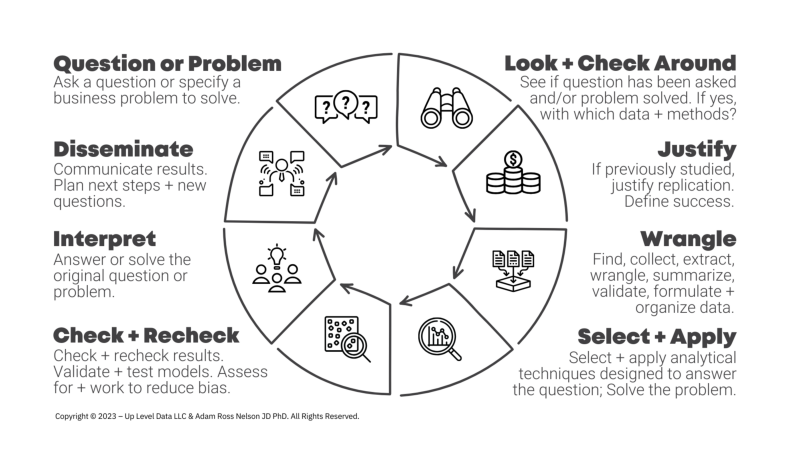
\includegraphics[keepaspectratio]{ParkSiteSelection_files/figure-pdf/fig-data-sicence-process-output-1.png}}

}

\caption{\label{fig-data-sicence-process}The data science process as
published in \emph{Confident Data Science} (Nelson, 2023).}

\end{figure}%

This process, as illustrated in Figure~\ref{fig-data-sicence-process}
starts at the upper left under the heading ``Question or Problem'' and
moves clockwise as an interative cycle as it also further consists of
the following:

\begin{enumerate}
\def\labelenumi{\arabic{enumi}.}
\tightlist
\item
  \textbf{State an analytical question or a business problem to solve.}
\item
  \textbf{Look + check around.} Explore if the question has been
  answered or if the problem has been solved. Also look to see what
  other similar questions or problems have been studied. Identify which
  methods have, or have not, been successful in the past. Also identify
  potential data sources.
\item
  \textbf{Justify the work.} Examine the scope of the question or the
  problem. Determine how answering the question or solving the problem
  provides value. Determine what additional revenues or efficiencies an
  answer to the question or a solution to the problem may bring. If the
  question has previously been answered or the problem previously solved
  decide if now is a good time to replicate the work (Is there now new
  data? Or, are there now new methods available?)
\item
  \textbf{Wrangle the data.} This involves finding, collecting,
  extracting, summarizing, validating, formulating, organizing,
  reshaping, coding, and recoding the data.
\item
  \textbf{Select and apply a method.} Determine which methods will best
  answer the analytical question or solve the business problem and then
  apply those methods.
\item
  \textbf{Check and recheck.} It is important to look back at this
  stage. Examine if the analytical question or business problem have
  been properly stated. Determine if there is new information that may
  have been missed, discounted, or overlooked in earlier stages. This
  stage may often involve seeking external input on in-progress work.
\item
  \textbf{Interpret the results.} Here the process involves answering
  the original analytical question or proffering a solution to the
  specified business problem.
\item
  \textbf{Dissemination.} The last stage involves either, or both
  disseminating the results or putting them into production.
\end{enumerate}

\subsection{Dissemination, Not
Production}\label{dissemination-not-production}

This paper's example does not exemplify putting a model into production.
Below is further explanation as to why putting a model into production
is not appropriate for this paper, and indeed the same is also true many
papers using data science's algorithmic mode of science.

This paper's environmental/limnological/geologic contexts are a primary
reason why the work here does not involve putting a model into
production. A model in production is useful when a business systems,
often driven by software systems, require a prediction that can serve as
a tool in making a decision. Or in contexts when information is
frequently or rapidly changing and the use case calls for using a
prediction as a recommendation or an automated decision.

\begin{tcolorbox}[enhanced jigsaw, coltitle=black, toprule=.15mm, arc=.35mm, bottomtitle=1mm, opacityback=0, leftrule=.75mm, left=2mm, colframe=quarto-callout-note-color-frame, toptitle=1mm, titlerule=0mm, breakable, colbacktitle=quarto-callout-note-color!10!white, colback=white, bottomrule=.15mm, title=\textcolor{quarto-callout-note-color}{\faInfo}\hspace{0.5em}{Note}, rightrule=.15mm, opacitybacktitle=0.6]

A model in production is most useful in environments where predictions
must be made repeatedly in response to rapidly changing data. These
contexts often involve automated systems or decision-making
pipelines---such as in weather forecasting, energy grid optimization, or
real-time environmental monitoring---where data streams update
frequently, and predictions must adapt continuously. For example, a
model deployed in production for natural resources management might
monitor streamflow or rainfall to inform automated alerts for flood
risks or fire danger. In such cases, real-time data ingestion and
dynamic model retraining are essential to the utility of the prediction.

\end{tcolorbox}

A description of Wisconsin's lakes from over fourty years ago remains as
true today as it was when first published. Lillie and Mason (1983)
describe the typical Wisconsin lake as ``natural in origin, equally
likely to be of seepage or drainage and stratified or mixed in basic
lake type and probably located in the northern half ot the state''
(p.~N).

In the case of Wisconsin's lakes it is not often that a new lake will
appear on the map. According to data utilized in this paper's analysis
from the WDNR there are \textbf{?var:number\_of\_lakes} lakes located
throughout the state of Wisconsin. The number of lakes has for decades
frequently been reported at a rounded 15,000 (Lillie and Mason (1983)).
The number of lakes in Wisconsin, or any geographic region, does not
change often. Thus, in this case it is sufficient to train and test a
model once on the existing data (which we do not expect to change
often).

\section{Data + Method}\label{data-method}

As discussed above the method for this project involves a one-time
analysis. Specifically the output will be a list of lakes that do have
public accommodations but are more similar to lakes that do not have
public accommodations (underserviced). A companion output will be a list
of lakes that do not have public accommodations but that are more
similar to lakes that do (overserviced).

Here I first discuss the data and then also the method that will produce
a list of lakes that should be further considered for the addition of
one or more public accommodation and a list of lakes that might benefit
from public accommodation closure or retirement.

\subsection{WDNR Data}\label{sec-wdnr-data}

The WDNR publishes the data for this analysis (Wisconsin Department of
Natural Resources 2024). The WDNR supports this data, uses it for a full
range of purposes (Natural Resources SWIMS Pages n.d.), and it receives
contributions from ``citizen science'' initiatives (Kretschmann et al.
2011).

\begin{Shaded}
\begin{Highlighting}[]
\NormalTok{df0.iloc[}\DecValTok{5194}\NormalTok{]}
\end{Highlighting}
\end{Shaded}

\begin{verbatim}
Waterbody ID Code (WBIC)                                              1605800
Lake Name                                                      Sevenmile Lake
Size (Acres)                                                            518.0
Official Max Depth                                                    43 FEET
Official Mean Depth                                                   19 FEET
Latitude                                                            45.879899
Longitude                                                          -89.051678
Public Landing                                                            Yes
Public Beach                                                               No
Public Park                                                               Yes
Fish Present                Musky, Panfish, Largemouth Bass, Smallmouth Ba...
Lake Type                                                            DRAINAGE
Water Clarity                                                        Moderate
County                                                         Oneida, Forest
Name: 5194, dtype: object
\end{verbatim}

\begin{Shaded}
\begin{Highlighting}[]
\NormalTok{characteristic\_lake\_id }\OperatorTok{=} \DecValTok{5194}

\ControlFlowTok{with} \BuiltInTok{open}\NormalTok{(}\StringTok{\textquotesingle{}\_variables.yml\textquotesingle{}}\NormalTok{, }\StringTok{\textquotesingle{}a\textquotesingle{}}\NormalTok{) }\ImportTok{as}\NormalTok{ f:}
    \CommentTok{\# Save characteristic lake name}
\NormalTok{    f.write(}\SpecialStringTok{f\textquotesingle{}char\_lake\_name: }\SpecialCharTok{\{}\NormalTok{df0}\SpecialCharTok{.}\NormalTok{iloc[characteristic\_lake\_id][}\StringTok{"Lake Name"}\NormalTok{]}\SpecialCharTok{\}}\CharTok{\textbackslash{}n}\SpecialStringTok{\textquotesingle{}}\NormalTok{)}
    \CommentTok{\# Save characteristic lake size}
\NormalTok{    f.write(}\SpecialStringTok{f\textquotesingle{}char\_lake\_size: }\SpecialCharTok{\{}\NormalTok{df0}\SpecialCharTok{.}\NormalTok{iloc[characteristic\_lake\_id][}\StringTok{"Size (Acres)"}\NormalTok{]}\SpecialCharTok{\}}\CharTok{\textbackslash{}n}\SpecialStringTok{\textquotesingle{}}\NormalTok{)}
    \CommentTok{\# Save characteristic lake max depth}
\NormalTok{    f.write(}\SpecialStringTok{f\textquotesingle{}char\_lake\_max\_depth: }\SpecialCharTok{\{}\NormalTok{df0}\SpecialCharTok{.}\NormalTok{iloc[characteristic\_lake\_id][}\StringTok{"Official Max Depth"}\NormalTok{]}\SpecialCharTok{.}\NormalTok{lower()}\SpecialCharTok{\}}\CharTok{\textbackslash{}n}\SpecialStringTok{\textquotesingle{}}\NormalTok{)}
    \CommentTok{\# Save characteristic lake mean depth}
\NormalTok{    f.write(}\SpecialStringTok{f\textquotesingle{}char\_lake\_mean\_depth: }\SpecialCharTok{\{}\NormalTok{df0}\SpecialCharTok{.}\NormalTok{iloc[characteristic\_lake\_id][}\StringTok{"Official Mean Depth"}\NormalTok{]}\SpecialCharTok{.}\NormalTok{lower()}\SpecialCharTok{\}}\CharTok{\textbackslash{}n}\SpecialStringTok{\textquotesingle{}}\NormalTok{)}
    \CommentTok{\# Save characteristic lake latitude}
\NormalTok{    f.write(}\SpecialStringTok{f\textquotesingle{}char\_lake\_latitude: }\SpecialCharTok{\{}\NormalTok{df0}\SpecialCharTok{.}\NormalTok{iloc[characteristic\_lake\_id][}\StringTok{"Latitude"}\NormalTok{]}\SpecialCharTok{\}}\CharTok{\textbackslash{}n}\SpecialStringTok{\textquotesingle{}}\NormalTok{)}
    \CommentTok{\# Save characteristic lake longitude}
\NormalTok{    f.write(}\SpecialStringTok{f\textquotesingle{}char\_lake\_longitude: }\SpecialCharTok{\{}\NormalTok{df0}\SpecialCharTok{.}\NormalTok{iloc[characteristic\_lake\_id][}\StringTok{"Longitude"}\NormalTok{]}\SpecialCharTok{\}}\CharTok{\textbackslash{}n}\SpecialStringTok{\textquotesingle{}}\NormalTok{)}
    \CommentTok{\# Save characteristic lake county}
\NormalTok{    f.write(}\SpecialStringTok{f\textquotesingle{}char\_lake\_county: }\SpecialCharTok{\{}\NormalTok{df0}\SpecialCharTok{.}\NormalTok{iloc[characteristic\_lake\_id][}\StringTok{"County"}\NormalTok{]}\SpecialCharTok{\}}\CharTok{\textbackslash{}n}\SpecialStringTok{\textquotesingle{}}\NormalTok{)}
\end{Highlighting}
\end{Shaded}

A characteristic lake in this data is \textbf{?var:char\_lake\_name}
which is about \textbf{?var:char\_lake\_size} in acres, up to
\textbf{?var:char\_lake\_max\_depth} deep, (with a mean depth of
\textbf{?var:char\_lake\_mean\_depth}), and located at
\textbf{?var:char\_lake\_latitude} latitude by
\textbf{?var:char\_lake\_longitude} longitude in
\textbf{?var:char\_lake\_county} counties.

This WDNR data features a high rate of missing data. A total of 6 of the
data's 14 columns contain some missing data.
Figure~\ref{fig-missing-data} displays missing data as bright lines in a
heatmap. Table~\ref{tbl-missing-data} shows the data's 6 columns with at
least some missing data. During data preparation, missing information
for the \texttt{lake\ type}, and \texttt{water\ clarity} will be
replaced with a new ``missing'' category. When creating a dummy array to
represent the \texttt{fish\ present} column records with missing data
will be represented by a set of \texttt{0} values. Missing data in the
\texttt{Official\ Max\ Depth} column will be replaced with data that is
a function of \texttt{Size\ (Acres)}. According to Lillie and Mason
(1983, 4) a Wisconsin lake's mean depth can be estimated as half of its
maximum depth. Accordingly, missing information in the
\texttt{Official\ Mean\ Depth} column will be replaced with 50\% of each
lake's maximum depth.

\begin{Shaded}
\begin{Highlighting}[]
\NormalTok{fig, ax }\OperatorTok{=}\NormalTok{ plt.subplots(figsize}\OperatorTok{=}\NormalTok{(}\DecValTok{6}\NormalTok{, }\DecValTok{3}\NormalTok{))}
\NormalTok{sns.set\_context(}\StringTok{\textquotesingle{}notebook\textquotesingle{}}\NormalTok{)}
\NormalTok{sns.heatmap(df0.transpose().isna())}
\end{Highlighting}
\end{Shaded}

\begin{figure}[H]

\centering{

\pandocbounded{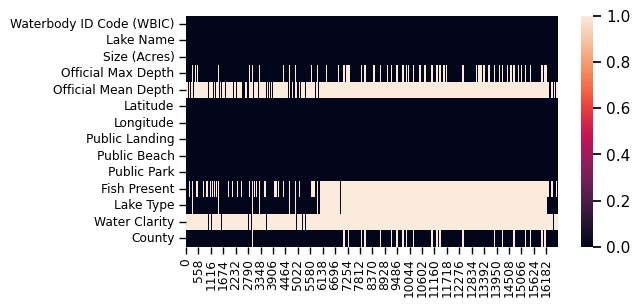
\includegraphics[keepaspectratio]{ParkSiteSelection_files/figure-pdf/fig-missing-data-output-1.png}}

}

\caption{\label{fig-missing-data}Heat map showing missing data. Bright
lines represent a mising data cell.}

\end{figure}%

\begin{Shaded}
\begin{Highlighting}[]
\CommentTok{\# Find the proportion of missing entries in each column.}
\NormalTok{missing\_table }\OperatorTok{=}\NormalTok{ pd.DataFrame(}
\NormalTok{    df0.isnull().mean(),}
    \CommentTok{\# Descriptively name the column}
\NormalTok{    columns}\OperatorTok{=}\NormalTok{[}\StringTok{"Proportion of Missing Data In Each Column"}\NormalTok{])}

\CommentTok{\# Filter to columns with missing data}
\NormalTok{missing\_table }\OperatorTok{=}\NormalTok{ missing\_table[}
\NormalTok{    missing\_table[}\StringTok{\textquotesingle{}Proportion of Missing Data In Each Column\textquotesingle{}}\NormalTok{] }\OperatorTok{\textgreater{}} \DecValTok{0}\NormalTok{]}

\CommentTok{\# Add more descriptive text to the table columns}
\NormalTok{missing\_table[}
\StringTok{\textquotesingle{}Proportion of Missing Data In Each Column\textquotesingle{}}\NormalTok{] }\OperatorTok{=}\NormalTok{ missing\_table[}
\StringTok{\textquotesingle{}Proportion of Missing Data In Each Column\textquotesingle{}}\NormalTok{].}\BuiltInTok{apply}\NormalTok{(}
    \KeywordTok{lambda}\NormalTok{ x: }\SpecialStringTok{f\textquotesingle{}}\SpecialCharTok{\{}\BuiltInTok{round}\NormalTok{(x }\OperatorTok{*} \DecValTok{100}\NormalTok{, }\DecValTok{2}\NormalTok{)}\SpecialCharTok{\}}\SpecialStringTok{ \% Missing Records\textquotesingle{}}\NormalTok{)}

\NormalTok{missing\_table}
\end{Highlighting}
\end{Shaded}

\begin{longtable}[]{@{}ll@{}}

\caption{\label{tbl-missing-data}The proportion of missing entries in
each column. Columns with no missing data not shown.}

\tabularnewline

\toprule\noalign{}
& Proportion of Missing Data In Each Column \\
\midrule\noalign{}
\endhead
\bottomrule\noalign{}
\endlastfoot
Official Max Depth & 19.94 \% Missing Records \\
Official Mean Depth & 90.18 \% Missing Records \\
Fish Present & 70.76 \% Missing Records \\
Lake Type & 62.24 \% Missing Records \\
Water Clarity & 96.23 \% Missing Records \\
County & 8.71 \% Missing Records \\

\end{longtable}

Below Figure~\ref{fig-wisconsin-lakes-mapped} shows the geographic
distribution of lakes across Wisconsin. The lakes with a public beach,
park, or boat landing show as dark \texttt{x} marks while the lakes with
no public beach, park, or boat landing show as small \texttt{o} marks.
Consistent with estimations from Lillie and Mason (1983) we see in
Figure~\ref{fig-wisconsin-lakes-mapped} that 50\% of Wiscosin's lakes
are above north 45.5 degress latitude.

\begin{Shaded}
\begin{Highlighting}[]
\CommentTok{\# Function to fetch and save Wisconsin GeoJSON if not present}
\KeywordTok{def}\NormalTok{ fetch\_wisconsin\_geojson(local\_path}\OperatorTok{=}\StringTok{"wisconsin.geojson"}\NormalTok{, verbose}\OperatorTok{=}\VariableTok{False}\NormalTok{):}
    \ControlFlowTok{if} \KeywordTok{not}\NormalTok{ os.path.exists(local\_path):}
        \ControlFlowTok{if}\NormalTok{ verbose: }\BuiltInTok{print}\NormalTok{(}\SpecialStringTok{f"}\SpecialCharTok{\{}\NormalTok{local\_path}\SpecialCharTok{\}}\SpecialStringTok{ not found. Downloading..."}\NormalTok{)}
\NormalTok{        web }\OperatorTok{=} \StringTok{\textquotesingle{}https://raw.githubusercontent.com\textquotesingle{}}
\NormalTok{        path }\OperatorTok{=} \StringTok{\textquotesingle{}glynnbird/usstatesgeojson/master/\textquotesingle{}}
        \BuiltInTok{file} \OperatorTok{=} \StringTok{\textquotesingle{}wisconsin.geojson\textquotesingle{}}
\NormalTok{        response }\OperatorTok{=}\NormalTok{ requests.get(web }\OperatorTok{+}\NormalTok{ path }\OperatorTok{+} \BuiltInTok{file}\NormalTok{)}
        \ControlFlowTok{if}\NormalTok{ response.status\_code }\OperatorTok{==} \DecValTok{200}\NormalTok{:}
            \ControlFlowTok{with} \BuiltInTok{open}\NormalTok{(local\_path, }\StringTok{\textquotesingle{}wb\textquotesingle{}}\NormalTok{) }\ImportTok{as} \BuiltInTok{file}\NormalTok{:}
                \BuiltInTok{file}\NormalTok{.write(response.content)}
            \ControlFlowTok{if}\NormalTok{ verbose: }\BuiltInTok{print}\NormalTok{(}\SpecialStringTok{f"Downloaded and saved }\SpecialCharTok{\{}\NormalTok{local\_path}\SpecialCharTok{\}}\SpecialStringTok{."}\NormalTok{)}
        \ControlFlowTok{else}\NormalTok{:}
\NormalTok{            fetch\_error }\OperatorTok{=} \SpecialStringTok{f"Wisconsin GeoJSON fetch failed. "}
\NormalTok{            fetch\_error }\OperatorTok{+=} \SpecialStringTok{f"HTTP status code: }\SpecialCharTok{\{}\NormalTok{response}\SpecialCharTok{.}\NormalTok{status\_code}\SpecialCharTok{\}}\SpecialStringTok{"}
            \ControlFlowTok{raise} \PreprocessorTok{ValueError}\NormalTok{(fetch\_error)}
    \ControlFlowTok{else}\NormalTok{:}
        \ControlFlowTok{if}\NormalTok{ verbose: }\BuiltInTok{print}\NormalTok{(}\SpecialStringTok{f"Using local copy of }\SpecialCharTok{\{}\NormalTok{local\_path}\SpecialCharTok{\}}\SpecialStringTok{."}\NormalTok{)}
    \ControlFlowTok{return}\NormalTok{ gpd.read\_file(local\_path)}

\CommentTok{\# Load Wisconsin GeoJSON}
\NormalTok{wisconsin }\OperatorTok{=}\NormalTok{ fetch\_wisconsin\_geojson()}

\CommentTok{\# Clean lake location data. Longitude sometimes stored as positive values.}
\NormalTok{lake\_data }\OperatorTok{=}\NormalTok{ df0[[}\StringTok{\textquotesingle{}Latitude\textquotesingle{}}\NormalTok{,}\StringTok{\textquotesingle{}Longitude\textquotesingle{}}\NormalTok{,}
                \StringTok{\textquotesingle{}Public Landing\textquotesingle{}}\NormalTok{,}\StringTok{\textquotesingle{}Public Beach\textquotesingle{}}\NormalTok{,}
                \StringTok{\textquotesingle{}Public Park\textquotesingle{}}\NormalTok{]].copy(deep}\OperatorTok{=}\VariableTok{True}\NormalTok{)}
\NormalTok{lake\_data[}\StringTok{\textquotesingle{}Longitude\textquotesingle{}}\NormalTok{] }\OperatorTok{=}\NormalTok{ [l }\ControlFlowTok{if}\NormalTok{ l }\OperatorTok{\textless{}} \DecValTok{0} \ControlFlowTok{else}\NormalTok{ l }\OperatorTok{*} \OperatorTok{{-}}\DecValTok{1} \ControlFlowTok{for}\NormalTok{ l }\KeywordTok{in}\NormalTok{ lake\_data[}\StringTok{\textquotesingle{}Longitude\textquotesingle{}}\NormalTok{]]}
\CommentTok{\# Remove records recording 0 Latitude}
\NormalTok{lake\_data }\OperatorTok{=}\NormalTok{ lake\_data[lake\_data[}\StringTok{\textquotesingle{}Latitude\textquotesingle{}}\NormalTok{] }\OperatorTok{\textgreater{}} \DecValTok{0}\NormalTok{]}

\CommentTok{\# Make hue for color code}
\NormalTok{lake\_data[}\StringTok{\textquotesingle{}Landing, Beach, or Park\textquotesingle{}}\NormalTok{] }\OperatorTok{=}\NormalTok{ lake\_data[}
\NormalTok{    [}\StringTok{\textquotesingle{}Public Landing\textquotesingle{}}\NormalTok{,}\StringTok{\textquotesingle{}Public Beach\textquotesingle{}}\NormalTok{,}\StringTok{\textquotesingle{}Public Park\textquotesingle{}}\NormalTok{]].}\BuiltInTok{max}\NormalTok{(axis}\OperatorTok{=}\DecValTok{1}\NormalTok{)}

\NormalTok{lake\_data[}\StringTok{\textquotesingle{}Landing, Beach, or Park\textquotesingle{}}\NormalTok{] }\OperatorTok{=}\NormalTok{ [}
    \StringTok{\textquotesingle{}Has Public Services\textquotesingle{}} \ControlFlowTok{if}\NormalTok{ i }\OperatorTok{==} \StringTok{"Yes"} 
    \ControlFlowTok{else} \StringTok{"Does Not Have Public Services"} \ControlFlowTok{for}\NormalTok{ i }\KeywordTok{in}\NormalTok{ lake\_data[}\StringTok{\textquotesingle{}Landing, Beach, or Park\textquotesingle{}}\NormalTok{]]}

\CommentTok{\# Convert lake data to GeoDataFrame}
\NormalTok{gdf\_lakes }\OperatorTok{=}\NormalTok{ gpd.GeoDataFrame(}
\NormalTok{    lake\_data, geometry}\OperatorTok{=}\NormalTok{gpd.points\_from\_xy(lake\_data.Longitude, lake\_data.Latitude)}
\NormalTok{)}

\CommentTok{\# Ensure both GeoDataFrames use the same CRS}
\NormalTok{gdf\_lakes.set\_crs(epsg}\OperatorTok{=}\DecValTok{4326}\NormalTok{, inplace}\OperatorTok{=}\VariableTok{True}\NormalTok{)}
\NormalTok{wisconsin }\OperatorTok{=}\NormalTok{ wisconsin.to\_crs(epsg}\OperatorTok{=}\DecValTok{4326}\NormalTok{)}

\CommentTok{\# Plotting}
\NormalTok{fig, ax }\OperatorTok{=}\NormalTok{ plt.subplots(figsize}\OperatorTok{=}\NormalTok{(}\DecValTok{10}\NormalTok{, }\DecValTok{8}\NormalTok{))}

\CommentTok{\# Plot Wisconsin outline}
\NormalTok{wisconsin.boundary.plot(ax}\OperatorTok{=}\NormalTok{ax, color}\OperatorTok{=}\StringTok{\textquotesingle{}black\textquotesingle{}}\NormalTok{, linewidth}\OperatorTok{=}\FloatTok{1.2}\NormalTok{)}

\CommentTok{\# Plot lake locations}
\NormalTok{sns.scatterplot(}
\NormalTok{    x}\OperatorTok{=}\StringTok{\textquotesingle{}Longitude\textquotesingle{}}\NormalTok{, y}\OperatorTok{=}\StringTok{\textquotesingle{}Latitude\textquotesingle{}}\NormalTok{, data}\OperatorTok{=}\NormalTok{lake\_data, ax}\OperatorTok{=}\NormalTok{ax,}
\NormalTok{    hue}\OperatorTok{=}\StringTok{\textquotesingle{}Landing, Beach, or Park\textquotesingle{}}\NormalTok{, style}\OperatorTok{=}\StringTok{\textquotesingle{}Landing, Beach, or Park\textquotesingle{}}\NormalTok{,}
\NormalTok{    markers}\OperatorTok{=}\NormalTok{\{}\StringTok{\textquotesingle{}Does Not Have Public Services\textquotesingle{}}\NormalTok{: }\StringTok{\textquotesingle{}o\textquotesingle{}}\NormalTok{, }\StringTok{\textquotesingle{}Has Public Services\textquotesingle{}}\NormalTok{: }\StringTok{\textquotesingle{}X\textquotesingle{}}\NormalTok{\},}
\NormalTok{    palette}\OperatorTok{=}\NormalTok{\{}\StringTok{\textquotesingle{}Does Not Have Public Services\textquotesingle{}}\NormalTok{: }\StringTok{\textquotesingle{}gray\textquotesingle{}}\NormalTok{, }\StringTok{\textquotesingle{}Has Public Services\textquotesingle{}}\NormalTok{: }\StringTok{\textquotesingle{}blue\textquotesingle{}}\NormalTok{\})}

\CommentTok{\# Set plot labels and title}
\NormalTok{ax.set\_title(}\StringTok{\textquotesingle{}Lakes in Wisconsin from WDNR SWIMS Data\textquotesingle{}}\NormalTok{)}
\NormalTok{ax.set\_xlabel(}\StringTok{\textquotesingle{}Longitude\textquotesingle{}}\NormalTok{)}
\NormalTok{ax.set\_ylabel(}\StringTok{\textquotesingle{}Latitude\textquotesingle{}}\NormalTok{)}

\NormalTok{plt.legend()}
\end{Highlighting}
\end{Shaded}

\begin{figure}[H]

\centering{

\pandocbounded{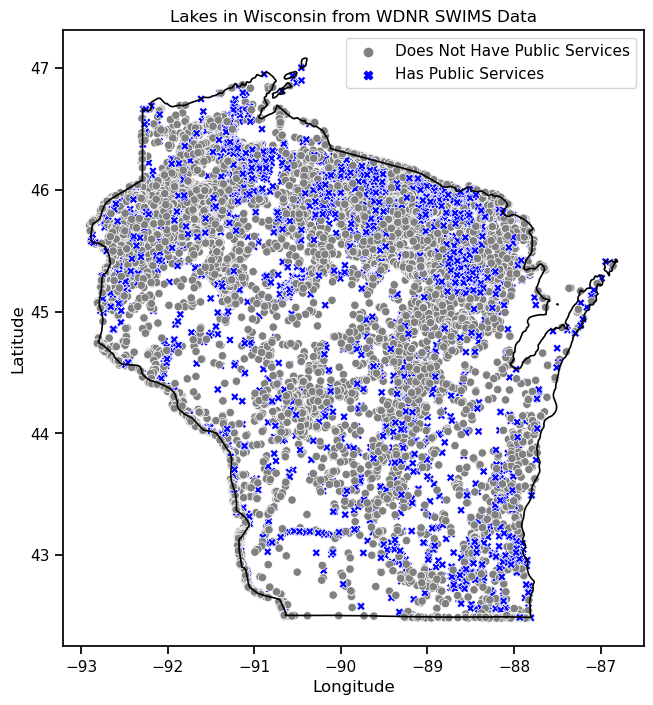
\includegraphics[keepaspectratio]{ParkSiteSelection_files/figure-pdf/fig-wisconsin-lakes-mapped-output-1.png}}

}

\caption{\label{fig-wisconsin-lakes-mapped}A map showing the location of
each lake in these data.}

\end{figure}%

\begin{tcolorbox}[enhanced jigsaw, coltitle=black, toprule=.15mm, arc=.35mm, bottomtitle=1mm, opacityback=0, leftrule=.75mm, left=2mm, colframe=quarto-callout-note-color-frame, toptitle=1mm, titlerule=0mm, breakable, colbacktitle=quarto-callout-note-color!10!white, colback=white, bottomrule=.15mm, title=\textcolor{quarto-callout-note-color}{\faInfo}\hspace{0.5em}{Note}, rightrule=.15mm, opacitybacktitle=0.6]

To create a geographic visualization of Wisconsin's lakes, this analysis
overlays lake location data onto a geospatial outline of the state. The
process relies on several essential tools and geospatial data formats,
including GeoJSON, GeoPandas, and the use of a coordinate reference
system (CRS) to ensure spatial consistency.

The geographic outline of Wisconsin is sourced from a publicly available
GeoJSON file hosted on GitHub. GeoJSON is a widely used format for
encoding geographic data structures using JSON (JavaScript Object
Notation). It stores spatial features such as points, lines, and
polygons along with associated attribute data. In this case, the polygon
defining the boundary of the state of Wisconsin is used as a background
layer in the final map.

I provide more thorough discussion of the processes and techniques for
building this map visual in the appendicies.

\end{tcolorbox}

\subsection{Preparation For Analysis}\label{preparation-for-analysis}

The following procedure prepares this data for analysis. Starting with a
fresh copy of the data from WDNR the code first reports a list of the
existing column names and then creates a new set of column names that
are more efficient to reference in code. When reviewing the first five
columns it appears that max depth and mean depth are stored as strings
and contain extraneous text (\texttt{"FEET"}) data. The code proceeds to
remove that extraneous text and then converts the data type to float.

For a more efficient analysis the code then converts the
\texttt{haslanding}, \texttt{hasbeach}, and \texttt{haspark} variables
to binary where a \texttt{1} replaces the WDNR provided \texttt{Yes}
value and a \texttt{0} replaces the WDNR provided \texttt{No} value. The
code also creates a \texttt{hasservice} variable that is a composite
which reports \texttt{1} if any of \texttt{haslanding},
\texttt{hasbeach}, or \texttt{haspark} are true and \texttt{0}
otherwise. The \texttt{hasservice} variable will be the primary outcome
variable in this analysis.

The code also inspects the \texttt{lat} and \texttt{long} data to
discover that some values are out of the expected possible range.
Wisconsin's southwest corner is at approxaibately 42.5°N by 92.89°W
while its northeast corner is at approxaimtely 47.1°N by 86.25°W. These
lake data from WDNR include values in the \texttt{lat} and \texttt{long}
columns beyond those ranges. As a preliminary step, where these WDNR
data report positive longitude the anlaysis assumes that the intended
value was negative to correspond with Wisconsin's location in the
western hemisphere. Upon converting the postive longitudinal data values
to negative, the remaining non-zero values fall within the expected
geographic range.

A total of \textbf{?var:zero\_coords\_count} records reported 0°, 0°
coordinates. The code also replaces these out of range 0°, 0° data with
longitude and latitude values associated with each lake's county
coordinates from gigasheet.com. A small number of records contained no
county data (or data from multiple counties) and thus the code drops
these remaining records from the analysis.

The newly renamed \texttt{fish} column contains a comma separated list
of fish species found in each lake. This column also contains a
gramatically correct ``and.'' To convert these fish data to an array of
dummy columns the code first replace the ``and'' with a comma via
\texttt{pd.str.replace(\textquotesingle{}\ and\textquotesingle{},\textquotesingle{},\textquotesingle{},\ \textquotesingle{})}
and then uses
\texttt{pd.str.get\_dummies(sep=\textquotesingle{},\ \textquotesingle{})}.

This code also manages missing data as described above in
Section~\ref{sec-wdnr-data} which describes the data as it was in its
oroginal form from WDNR. Three extrememly large lakes in the .018th
percential including Lake Winebago are removed. A final inspection of
summary statistics is provided in Table~\ref{tbl-prepared-summary}.

\begin{Shaded}
\begin{Highlighting}[]
\CommentTok{\# Start with a fresh copy of the data from WDNR}
\NormalTok{df }\OperatorTok{=}\NormalTok{ pd.read\_csv(}\StringTok{\textquotesingle{}Lakes\_Original.csv\textquotesingle{}}\NormalTok{)}

\NormalTok{original\_rows, original\_cols }\OperatorTok{=}\NormalTok{ df.shape}

\CommentTok{\# Write original column and record shape for later reference}
\ControlFlowTok{with} \BuiltInTok{open}\NormalTok{(}\StringTok{"\_variables.yml"}\NormalTok{, }\StringTok{"a"}\NormalTok{) }\ImportTok{as}\NormalTok{ f:}
\NormalTok{    f.write(}\SpecialStringTok{f"original\_rows\_count: }\SpecialCharTok{\{}\NormalTok{original\_rows}\SpecialCharTok{\}}\CharTok{\textbackslash{}n}\SpecialStringTok{"}\NormalTok{)}
\NormalTok{    f.write(}\SpecialStringTok{f"original\_cols\_count: }\SpecialCharTok{\{}\NormalTok{original\_cols}\SpecialCharTok{\}}\CharTok{\textbackslash{}n}\SpecialStringTok{"}\NormalTok{)}

\CommentTok{\# Produce a list of columns}
\BuiltInTok{print}\NormalTok{(}\StringTok{\textquotesingle{}Initial Column Set:\textquotesingle{}}\NormalTok{)}
\BuiltInTok{print}\NormalTok{(df.columns, end}\OperatorTok{=}\StringTok{\textquotesingle{}}\CharTok{\textbackslash{}n\textbackslash{}n\textbackslash{}n}\StringTok{\textquotesingle{}}\NormalTok{)}

\CommentTok{\# Rename columns for quicker reference}
\NormalTok{df.columns }\OperatorTok{=}\NormalTok{ [}\StringTok{\textquotesingle{}ID\textquotesingle{}}\NormalTok{,}\StringTok{\textquotesingle{}name\textquotesingle{}}\NormalTok{,}\StringTok{\textquotesingle{}size\textquotesingle{}}\NormalTok{,}\StringTok{\textquotesingle{}maxdepth\textquotesingle{}}\NormalTok{,}
              \StringTok{\textquotesingle{}meandepth\textquotesingle{}}\NormalTok{,}\StringTok{\textquotesingle{}lat\textquotesingle{}}\NormalTok{,}\StringTok{\textquotesingle{}lon\textquotesingle{}}\NormalTok{,}
              \StringTok{\textquotesingle{}haslanding\textquotesingle{}}\NormalTok{,}\StringTok{\textquotesingle{}hasbeach\textquotesingle{}}\NormalTok{,}\StringTok{\textquotesingle{}haspark\textquotesingle{}}\NormalTok{,}
              \StringTok{\textquotesingle{}fish\textquotesingle{}}\NormalTok{,}\StringTok{\textquotesingle{}type\textquotesingle{}}\NormalTok{,}\StringTok{\textquotesingle{}clarity\textquotesingle{}}\NormalTok{,}\StringTok{\textquotesingle{}county\textquotesingle{}}\NormalTok{]}

\CommentTok{\# Review sample of first 5 columns}
\BuiltInTok{print}\NormalTok{(}\StringTok{\textquotesingle{}Sample, first five columns before modifications:\textquotesingle{}}\NormalTok{)}
\BuiltInTok{print}\NormalTok{(df[df.columns[:}\DecValTok{5}\NormalTok{]].sample(}\DecValTok{4}\NormalTok{), end}\OperatorTok{=}\StringTok{\textquotesingle{}}\CharTok{\textbackslash{}n\textbackslash{}n\textbackslash{}n}\StringTok{\textquotesingle{}}\NormalTok{)}

\CommentTok{\# Convert maxdepth, meandepth to numberic}
\NormalTok{df[}\StringTok{\textquotesingle{}maxdepth\textquotesingle{}}\NormalTok{] }\OperatorTok{=}\NormalTok{ df[}\StringTok{\textquotesingle{}maxdepth\textquotesingle{}}\NormalTok{].}\BuiltInTok{str}\NormalTok{.replace(}\StringTok{\textquotesingle{} FEET\textquotesingle{}}\NormalTok{,}\StringTok{\textquotesingle{}\textquotesingle{}}\NormalTok{).astype(}\StringTok{\textquotesingle{}float\textquotesingle{}}\NormalTok{)}
\NormalTok{df[}\StringTok{\textquotesingle{}meandepth\textquotesingle{}}\NormalTok{] }\OperatorTok{=}\NormalTok{ df[}\StringTok{\textquotesingle{}meandepth\textquotesingle{}}\NormalTok{].}\BuiltInTok{str}\NormalTok{.replace(}\StringTok{\textquotesingle{} FEET\textquotesingle{}}\NormalTok{,}\StringTok{\textquotesingle{}\textquotesingle{}}\NormalTok{).astype(}\StringTok{\textquotesingle{}float\textquotesingle{}}\NormalTok{)}
\CommentTok{\# Find imputation function for maxdepth}
\NormalTok{maxdepth\_imputation }\OperatorTok{=}\NormalTok{ df[[}\StringTok{\textquotesingle{}maxdepth\textquotesingle{}}\NormalTok{,}\StringTok{\textquotesingle{}size\textquotesingle{}}\NormalTok{]].dropna()}
\NormalTok{maxdepth\_imputation }\OperatorTok{=}\NormalTok{ df[}\StringTok{\textquotesingle{}maxdepth\textquotesingle{}}\NormalTok{].mean() }\OperatorTok{/}\NormalTok{ df[}\StringTok{\textquotesingle{}size\textquotesingle{}}\NormalTok{].mean()}

\CommentTok{\# Tag records that had missing max depth}
\NormalTok{df[}\StringTok{\textquotesingle{}maxdepth\_missing\textquotesingle{}}\NormalTok{] }\OperatorTok{=}\NormalTok{ (df[}\StringTok{\textquotesingle{}maxdepth\textquotesingle{}}\NormalTok{].fillna(}\DecValTok{999999}\NormalTok{) }\OperatorTok{==} \DecValTok{999999}\NormalTok{) }\OperatorTok{*} \DecValTok{1}
\CommentTok{\# Apply imputation function to missing maxdepth entries}
\NormalTok{df[}\StringTok{\textquotesingle{}maxdepth\textquotesingle{}}\NormalTok{] }\OperatorTok{=}\NormalTok{ df[}\StringTok{\textquotesingle{}maxdepth\textquotesingle{}}\NormalTok{].fillna(df[}\StringTok{\textquotesingle{}size\textquotesingle{}}\NormalTok{] }\OperatorTok{*}\NormalTok{ maxdepth\_imputation)}

\CommentTok{\# Tag records that were missing meandepth}
\NormalTok{df[}\StringTok{\textquotesingle{}meandepth\_missing\textquotesingle{}}\NormalTok{] }\OperatorTok{=}\NormalTok{ (df[}\StringTok{\textquotesingle{}meandepth\textquotesingle{}}\NormalTok{].fillna(}\DecValTok{999999}\NormalTok{) }\OperatorTok{==} \DecValTok{999999}\NormalTok{) }\OperatorTok{*} \DecValTok{1}
\CommentTok{\# Apply imputation function to missing meandepth entries}
\NormalTok{df[}\StringTok{\textquotesingle{}meandepth\textquotesingle{}}\NormalTok{] }\OperatorTok{=}\NormalTok{ df[}\StringTok{\textquotesingle{}meandepth\textquotesingle{}}\NormalTok{].fillna(df[}\StringTok{\textquotesingle{}maxdepth\textquotesingle{}}\NormalTok{] }\OperatorTok{*} \FloatTok{.5}\NormalTok{)}

\CommentTok{\# Print heading for notebook output}
\BuiltInTok{print}\NormalTok{(}\StringTok{\textquotesingle{}Display excerpt of modified data.\textquotesingle{}}\NormalTok{)}

\CommentTok{\# Check results (first 5 columns)}
\BuiltInTok{print}\NormalTok{(df[df.columns[:}\DecValTok{5}\NormalTok{]].sample(}\DecValTok{4}\NormalTok{))}

\CommentTok{\# Check results (next 5 columns)}
\BuiltInTok{print}\NormalTok{(df[df.columns[}\DecValTok{5}\NormalTok{:}\DecValTok{10}\NormalTok{]].sample(}\DecValTok{4}\NormalTok{))}

\CommentTok{\# Check results (remaining columns)}
\BuiltInTok{print}\NormalTok{(df[df.columns[}\DecValTok{10}\NormalTok{:]].sample(}\DecValTok{4}\NormalTok{), end}\OperatorTok{=}\StringTok{\textquotesingle{}}\CharTok{\textbackslash{}n\textbackslash{}n\textbackslash{}n}\StringTok{\textquotesingle{}}\NormalTok{)}

\CommentTok{\# Dummy encode the \textquotesingle{}haslanding\textquotesingle{},\textquotesingle{}hasbeach\textquotesingle{},\textquotesingle{}haspark\textquotesingle{} variables}
\ControlFlowTok{for}\NormalTok{ col }\KeywordTok{in}\NormalTok{ [}\StringTok{\textquotesingle{}haslanding\textquotesingle{}}\NormalTok{,}\StringTok{\textquotesingle{}hasbeach\textquotesingle{}}\NormalTok{,}\StringTok{\textquotesingle{}haspark\textquotesingle{}}\NormalTok{]:}
\NormalTok{    df[col] }\OperatorTok{=}\NormalTok{ [}\DecValTok{1} \ControlFlowTok{if}\NormalTok{ c }\OperatorTok{==} \StringTok{"Yes"} \ControlFlowTok{else} \DecValTok{0} \ControlFlowTok{for}\NormalTok{ c }\KeywordTok{in}\NormalTok{ df[col]]}

\CommentTok{\# Create a composit hasservice variable}
\NormalTok{df[}\StringTok{\textquotesingle{}hasservice\textquotesingle{}}\NormalTok{] }\OperatorTok{=}\NormalTok{ df[[}\StringTok{\textquotesingle{}haslanding\textquotesingle{}}\NormalTok{,}\StringTok{\textquotesingle{}hasbeach\textquotesingle{}}\NormalTok{,}\StringTok{\textquotesingle{}haspark\textquotesingle{}}\NormalTok{]].}\BuiltInTok{max}\NormalTok{(axis}\OperatorTok{=}\DecValTok{1}\NormalTok{)}

\CommentTok{\# Convert positive longitudinal values to negative}
\NormalTok{df[}\StringTok{\textquotesingle{}lon\textquotesingle{}}\NormalTok{] }\OperatorTok{=}\NormalTok{ [l }\ControlFlowTok{if}\NormalTok{ l }\OperatorTok{\textless{}} \DecValTok{0} \ControlFlowTok{else}\NormalTok{ l }\OperatorTok{*} \OperatorTok{{-}}\DecValTok{1} \ControlFlowTok{for}\NormalTok{ l }\KeywordTok{in}\NormalTok{ df[}\StringTok{\textquotesingle{}lon\textquotesingle{}}\NormalTok{]]}
\CommentTok{\# Replace 0, 0 coordinates with county coordiantes from gigasheet.com}
\NormalTok{county\_list }\OperatorTok{=}\NormalTok{ pd.read\_csv(}\StringTok{\textquotesingle{}gigsheet{-}counties.csv\textquotesingle{}}\NormalTok{)}
\CommentTok{\# Create a county to lon mapper}
\NormalTok{lon\_map }\OperatorTok{=} \BuiltInTok{dict}\NormalTok{(}\BuiltInTok{zip}\NormalTok{(county\_list[}\StringTok{\textquotesingle{}name\textquotesingle{}}\NormalTok{], county\_list[}\StringTok{\textquotesingle{}lng\textquotesingle{}}\NormalTok{]))}
\CommentTok{\# Create a county to lon mapper}
\NormalTok{lat\_map }\OperatorTok{=} \BuiltInTok{dict}\NormalTok{(}\BuiltInTok{zip}\NormalTok{(county\_list[}\StringTok{\textquotesingle{}name\textquotesingle{}}\NormalTok{], county\_list[}\StringTok{\textquotesingle{}lat\textquotesingle{}}\NormalTok{]))}

\CommentTok{\# Apply the longitude mapper}
\NormalTok{df[}\StringTok{\textquotesingle{}lon\textquotesingle{}}\NormalTok{] }\OperatorTok{=}\NormalTok{ pd.Series(np.where(}
\NormalTok{    df[}\StringTok{\textquotesingle{}lon\textquotesingle{}}\NormalTok{] }\OperatorTok{==} \DecValTok{0}\NormalTok{, df[}\StringTok{\textquotesingle{}county\textquotesingle{}}\NormalTok{].}\BuiltInTok{map}\NormalTok{(lon\_map), df[}\StringTok{\textquotesingle{}lon\textquotesingle{}}\NormalTok{])).fillna(}\DecValTok{0}\NormalTok{)}
\CommentTok{\# Apply the latitude mapper}
\NormalTok{df[}\StringTok{\textquotesingle{}lat\textquotesingle{}}\NormalTok{] }\OperatorTok{=}\NormalTok{ pd.Series(np.where(}
\NormalTok{    df[}\StringTok{\textquotesingle{}lat\textquotesingle{}}\NormalTok{] }\OperatorTok{==} \DecValTok{0}\NormalTok{, df[}\StringTok{\textquotesingle{}county\textquotesingle{}}\NormalTok{].}\BuiltInTok{map}\NormalTok{(lat\_map), df[}\StringTok{\textquotesingle{}lat\textquotesingle{}}\NormalTok{])).fillna(}\DecValTok{0}\NormalTok{)}

\CommentTok{\# Remove remaining records recording 0°, 0° coords (appox 7 records)}
\NormalTok{df }\OperatorTok{=}\NormalTok{ df[df[}\StringTok{\textquotesingle{}lat\textquotesingle{}}\NormalTok{] }\OperatorTok{\textgreater{}} \DecValTok{0}\NormalTok{]}

\CommentTok{\# Remove and replace extraneous "and" from fish column}
\NormalTok{df[}\StringTok{\textquotesingle{}fish\textquotesingle{}}\NormalTok{] }\OperatorTok{=}\NormalTok{ df[}\StringTok{\textquotesingle{}fish\textquotesingle{}}\NormalTok{].}\BuiltInTok{str}\NormalTok{.replace(}\StringTok{\textquotesingle{} and \textquotesingle{}}\NormalTok{,}\StringTok{\textquotesingle{}, \textquotesingle{}}\NormalTok{)}
\CommentTok{\# Convert fish to dummy array and join}
\NormalTok{df }\OperatorTok{=}\NormalTok{ df.join(df[}\StringTok{\textquotesingle{}fish\textquotesingle{}}\NormalTok{].}\BuiltInTok{str}\NormalTok{.get\_dummies(sep}\OperatorTok{=}\StringTok{\textquotesingle{}, \textquotesingle{}}\NormalTok{))}
\CommentTok{\# Discard original raw data}
\NormalTok{df }\OperatorTok{=}\NormalTok{ df.drop(}\StringTok{\textquotesingle{}fish\textquotesingle{}}\NormalTok{, axis}\OperatorTok{=}\DecValTok{1}\NormalTok{)}

\CommentTok{\# Create "Missing" category for nominal type and clarity}
\NormalTok{df[}\StringTok{\textquotesingle{}type\textquotesingle{}}\NormalTok{] }\OperatorTok{=}\NormalTok{ df[}\StringTok{\textquotesingle{}type\textquotesingle{}}\NormalTok{].fillna(}\StringTok{\textquotesingle{}Missing\textquotesingle{}}\NormalTok{)}
\NormalTok{df[}\StringTok{\textquotesingle{}clarity\textquotesingle{}}\NormalTok{] }\OperatorTok{=}\NormalTok{ df[}\StringTok{\textquotesingle{}clarity\textquotesingle{}}\NormalTok{].fillna(}\StringTok{\textquotesingle{}Missing\textquotesingle{}}\NormalTok{)}

\CommentTok{\# Count number of lakes with m ore than 20,000 acres}
\BuiltInTok{print}\NormalTok{(}\SpecialStringTok{f"There are }\SpecialCharTok{\{}\BuiltInTok{len}\NormalTok{(df[df[}\StringTok{\textquotesingle{}size\textquotesingle{}}\NormalTok{] }\OperatorTok{\textgreater{}} \DecValTok{20000}\NormalTok{])}\SpecialCharTok{\}}\SpecialStringTok{ lakes greater than 20,000 acres"}\NormalTok{)}

\CommentTok{\# Remove lakes more than 20,000 acres}
\NormalTok{df }\OperatorTok{=}\NormalTok{ df[df[}\StringTok{\textquotesingle{}size\textquotesingle{}}\NormalTok{] }\OperatorTok{\textless{}} \DecValTok{20000}\NormalTok{]}
\end{Highlighting}
\end{Shaded}

\subsection{Exploratory Data Analysis}\label{exploratory-data-analysis}

Exploratory Data Analysis (EDA) serves as a critical bridge between raw
data and later more formal analysis and data modeling. This EDA is the
stage at which a scientist engages directly with data to uncover initial
patterns, surface anomalies, identify missing values, and begin
assessing the structure and relationships among variables. Gutman and
Goldmeier (2021) describe exploratory data analysis as ``an ongoing
process'' (p.~52). Thus EDA is not merely a preliminary step, but rather
a dynamic and iterative component of the broader data science workflow.
This ongoing process allows the analyst to refine questions, revisit
assumptions, and incrementally develop insight into the nature and
quality of the data.

As Nelson (2023) notes, ``without at least some preparation, an
exploratory analysis might reveal less than fully useful insights.
Simultaneously, without at least some exploration it is not fully
possible to know what preparation will be necessary before a full
analysis'' (p.~85). This is a \emph{which comes first} problem; a
proverbial \emph{chicken or egg} question. For example, in this paper a
handful of data manipulations have already been described and executed
above, all of which required at least some exploration. Proper execution
of EDA early and often through the course of a project guides both data
preparation and the analysis along the way. Below is a more formal and
analytical exploration of the data aimed at understanding which features
may be useful in a predictive algorithm.

\begin{Shaded}
\begin{Highlighting}[]
\CommentTok{\# Preserve summary statistics for later reference in the appendix}
\NormalTok{summary\_stats\_appendix }\OperatorTok{=}\NormalTok{ df.drop(}
\NormalTok{    [}\StringTok{\textquotesingle{}ID\textquotesingle{}}\NormalTok{,}\StringTok{\textquotesingle{}haslanding\textquotesingle{}}\NormalTok{,}\StringTok{\textquotesingle{}hasbeach\textquotesingle{}}\NormalTok{,}\StringTok{\textquotesingle{}haspark\textquotesingle{}}\NormalTok{], }
\NormalTok{    axis}\OperatorTok{=}\DecValTok{1}\NormalTok{).describe().}\BuiltInTok{round}\NormalTok{(}\DecValTok{3}\NormalTok{).transpose().drop([}\StringTok{\textquotesingle{}25\%\textquotesingle{}}\NormalTok{,}\StringTok{\textquotesingle{}75\%\textquotesingle{}}\NormalTok{], axis}\OperatorTok{=}\DecValTok{1}\NormalTok{)}

\NormalTok{summary\_stats }\OperatorTok{=}\NormalTok{ df.drop(}
\NormalTok{    [}\StringTok{\textquotesingle{}ID\textquotesingle{}}\NormalTok{,}\StringTok{\textquotesingle{}haslanding\textquotesingle{}}\NormalTok{,}\StringTok{\textquotesingle{}hasbeach\textquotesingle{}}\NormalTok{,}\StringTok{\textquotesingle{}haspark\textquotesingle{}}\NormalTok{], axis}\OperatorTok{=}\DecValTok{1}\NormalTok{)}

\NormalTok{summary\_has }\OperatorTok{=}\NormalTok{ summary\_stats[}
\NormalTok{    summary\_stats[}\StringTok{\textquotesingle{}hasservice\textquotesingle{}}\NormalTok{] }\OperatorTok{==} \DecValTok{1}\NormalTok{].describe().transpose()[}
\NormalTok{        [}\StringTok{\textquotesingle{}mean\textquotesingle{}}\NormalTok{,}\StringTok{\textquotesingle{}std\textquotesingle{}}\NormalTok{]]}
\NormalTok{summary\_has\_n }\OperatorTok{=}\NormalTok{ summary\_stats[summary\_stats[}\StringTok{\textquotesingle{}hasservice\textquotesingle{}}\NormalTok{]}\OperatorTok{==}\DecValTok{1}\NormalTok{].shape[}\DecValTok{0}\NormalTok{]}

\NormalTok{summary\_has\_not }\OperatorTok{=}\NormalTok{ summary\_stats[}
\NormalTok{    summary\_stats[}\StringTok{\textquotesingle{}hasservice\textquotesingle{}}\NormalTok{] }\OperatorTok{==} \DecValTok{0}\NormalTok{].describe().transpose()[}
\NormalTok{        [}\StringTok{\textquotesingle{}mean\textquotesingle{}}\NormalTok{,}\StringTok{\textquotesingle{}std\textquotesingle{}}\NormalTok{]]}
\NormalTok{summary\_has\_not\_n }\OperatorTok{=}\NormalTok{ summary\_stats[summary\_stats[}\StringTok{\textquotesingle{}hasservice\textquotesingle{}}\NormalTok{]}\OperatorTok{==}\DecValTok{0}\NormalTok{].shape[}\DecValTok{0}\NormalTok{]}

\NormalTok{summary\_all }\OperatorTok{=}\NormalTok{ summary\_stats.describe().transpose()[}
\NormalTok{    [}\StringTok{\textquotesingle{}mean\textquotesingle{}}\NormalTok{,}\StringTok{\textquotesingle{}std\textquotesingle{}}\NormalTok{]]}
\NormalTok{summary\_all\_n }\OperatorTok{=}\NormalTok{ summary\_stats.shape[}\DecValTok{0}\NormalTok{]}

\NormalTok{summary\_stats\_final }\OperatorTok{=}\NormalTok{ pd.concat([summary\_has, summary\_has\_not, }
\NormalTok{           summary\_all], axis}\OperatorTok{=}\DecValTok{1}\NormalTok{, }
\NormalTok{           keys}\OperatorTok{=}\NormalTok{[}\SpecialStringTok{f\textquotesingle{}Has Service n=}\SpecialCharTok{\{}\NormalTok{summary\_has\_n}\SpecialCharTok{\}}\SpecialStringTok{\textquotesingle{}}\NormalTok{,}
                 \SpecialStringTok{f\textquotesingle{}No Service n=}\SpecialCharTok{\{}\NormalTok{summary\_has\_not\_n}\SpecialCharTok{\}}\SpecialStringTok{\textquotesingle{}}\NormalTok{,}
                 \SpecialStringTok{f\textquotesingle{}Pooled Stats n=}\SpecialCharTok{\{}\NormalTok{summary\_all\_n}\SpecialCharTok{\}}\SpecialStringTok{\textquotesingle{}}\NormalTok{])}

\NormalTok{summary\_stats\_final.drop([}\StringTok{\textquotesingle{}hasservice\textquotesingle{}}\NormalTok{])}
\end{Highlighting}
\end{Shaded}

\begin{longtable}[]{@{}lllllll@{}}

\caption{\label{tbl-prepared-summary}Summary statistics following data
preparation.}

\tabularnewline

\toprule\noalign{}
& \multicolumn{2}{l}{%
Has Service n=5412} & \multicolumn{2}{l}{%
No Service n=11289} & \multicolumn{2}{l@{}}{%
Pooled Stats n=16701} \\
& mean & std & mean & std & mean & std \\
\midrule\noalign{}
\endhead
\bottomrule\noalign{}
\endlastfoot
size & 126.103186 & 620.251559 & 15.566853 & 72.814624 & 51.386422 &
361.816980 \\
maxdepth & 18.030048 & 34.543742 & 10.388841 & 15.992963 & 12.864993 &
23.922990 \\
meandepth & 8.347434 & 16.790334 & 5.121726 & 7.871674 & 6.167024 &
11.640702 \\
lat & 45.362475 & 0.960428 & 45.195551 & 0.960455 & 45.249643 &
0.963590 \\
lon & -90.031606 & 1.301074 & -90.318745 & 1.356957 & -90.225697 &
1.345791 \\
maxdepth\_missing & 0.105876 & 0.307707 & 0.243954 & 0.429484 & 0.199210
& 0.399418 \\
meandepth\_missing & 0.772358 & 0.419349 & 0.963770 & 0.186870 &
0.901742 & 0.297672 \\
Catfish & 0.013304 & 0.114583 & 0.002480 & 0.049743 & 0.005988 &
0.077150 \\
Largemouth Bass & 0.407428 & 0.491401 & 0.148729 & 0.355837 & 0.232561 &
0.422477 \\
Musky & 0.097746 & 0.296998 & 0.016831 & 0.128642 & 0.043051 &
0.202979 \\
Northern Pike & 0.296748 & 0.456867 & 0.084418 & 0.278027 & 0.153224 &
0.360214 \\
Panfish & 0.445122 & 0.497025 & 0.180087 & 0.384277 & 0.265972 &
0.441863 \\
Smallmouth Bass & 0.092018 & 0.289078 & 0.017628 & 0.131600 & 0.041734 &
0.199987 \\
Sturgeon & 0.007761 & 0.087759 & 0.000443 & 0.021042 & 0.002814 &
0.052976 \\
Trout & 0.060791 & 0.238968 & 0.019311 & 0.137621 & 0.032753 &
0.177994 \\
Walleye & 0.161493 & 0.368019 & 0.026220 & 0.159797 & 0.070056 &
0.255248 \\

\end{longtable}

\textbf{TODO: Add remaining columns to this table. See page 20ish.}

Table~\ref{tbl-prepared-summary} presents summary statistics for these
lakes data from the WDNR, segmented by whether or not the lake has
public services (boat landing, beach, or park). The table reports the
mean and standard deviation for each variable within both groups in the
left and middle columns, along with pooled overall statistics on the two
far right columns. This table provides a summary that can assist in
evaluating which variables may serve as useful predictors in classifying
or predicting whether a lake has public services.

For example, lakes with public services are, on average, much larger
than lakes without services (126.1 vs.~15.6 acres), and the pooled mean
is 51.4 acres. The standard deviation is also substantially higher among
lakes with services, reflecting greater variability in size. This
difference suggests that lake size may be a strong candidate as a
predictive variable, with larger lakes being much more likely to have
public accommodations. Similarly maximum depth (maxdepth), mean depth
(meandepth), along with the presence of some fish speacies may also
offer predictive value.

The final data set consists of 16701 records and 25 columns; there are
no missing data. The primary target in this paper's analysis is whether
the lake has a public service such as a boat landing, beach, or park.
Approximately 32.41\% of these lakes have at least one public service.

\subsection{Visual Exploratory Data
Analysis}\label{visual-exploratory-data-analysis}

To explore how each variable may predict the presence of a public
service on any of Wisconsin's lakes I produce series of categorical
violine plots in Figure~\ref{fig-violin-plot}. This figure further
illustrats how the presence of public services such as boat landings,
beaches, or parks may relate to five continuous features of each lake:
size, maximum depth, mean depth, latitude, and longitude. Each plot
shows the distribution of these features' natural log values for lakes
with and without public services.

\begin{Shaded}
\begin{Highlighting}[]
\CommentTok{\# Create a grid of subplots}
\NormalTok{fig, axes }\OperatorTok{=}\NormalTok{ plt.subplots(}
\NormalTok{    figsize}\OperatorTok{=}\NormalTok{(}\DecValTok{12}\NormalTok{, }\DecValTok{20}\NormalTok{),}
\NormalTok{    ncols}\OperatorTok{=}\DecValTok{1}\NormalTok{, nrows}\OperatorTok{=}\DecValTok{5}\NormalTok{,}
\NormalTok{    squeeze}\OperatorTok{=}\VariableTok{False}\NormalTok{)}

\NormalTok{axes }\OperatorTok{=}\NormalTok{ axes.flatten() }\ControlFlowTok{if} \BuiltInTok{isinstance}\NormalTok{(axes, np.ndarray) }\ControlFlowTok{else}\NormalTok{ [axes]}

\CommentTok{\# Adjust the spacing between the subplots}
\NormalTok{plt.subplots\_adjust(hspace}\OperatorTok{=}\FloatTok{0.5}\NormalTok{, wspace}\OperatorTok{=}\FloatTok{0.3}\NormalTok{)}

\CommentTok{\# Tuple list of var names and titles}
\NormalTok{variables }\OperatorTok{=}\NormalTok{ [}
\NormalTok{    (}\StringTok{\textquotesingle{}size\textquotesingle{}}\NormalTok{, }\StringTok{\textquotesingle{}Size in acres\textquotesingle{}}\NormalTok{),}
\NormalTok{    (}\StringTok{\textquotesingle{}maxdepth\textquotesingle{}}\NormalTok{, }\StringTok{\textquotesingle{}Maximum lake depth\textquotesingle{}}\NormalTok{),}
\NormalTok{    (}\StringTok{\textquotesingle{}meandepth\textquotesingle{}}\NormalTok{, }\StringTok{\textquotesingle{}Mean lake depth\textquotesingle{}}\NormalTok{),}
\NormalTok{    (}\StringTok{\textquotesingle{}lat\textquotesingle{}}\NormalTok{, }\StringTok{\textquotesingle{}Latitude location\textquotesingle{}}\NormalTok{),}
\NormalTok{    (}\StringTok{\textquotesingle{}lon\textquotesingle{}}\NormalTok{, }\StringTok{\textquotesingle{}Longitude Location\textquotesingle{}}\NormalTok{)}
\NormalTok{]}

\CommentTok{\# Iterate through list of variables and titles}
\ControlFlowTok{for}\NormalTok{ i, (var, title) }\KeywordTok{in} \BuiltInTok{enumerate}\NormalTok{(variables):}
\NormalTok{    sns.violinplot(data}\OperatorTok{=}\NormalTok{df, x}\OperatorTok{=}\NormalTok{np.log(np.}\BuiltInTok{abs}\NormalTok{(df[var])), }
\NormalTok{                   y}\OperatorTok{=}\StringTok{\textquotesingle{}hasservice\textquotesingle{}}\NormalTok{, orient}\OperatorTok{=}\StringTok{\textquotesingle{}h\textquotesingle{}}\NormalTok{, }
\NormalTok{                   ax}\OperatorTok{=}\NormalTok{axes[i])}
\NormalTok{    axes[i].set\_title(}\SpecialStringTok{f\textquotesingle{}}\SpecialCharTok{\{}\NormalTok{title}\SpecialCharTok{\}}\SpecialStringTok{ (Fig 4}\SpecialCharTok{\{}\StringTok{"abcde"}\NormalTok{[i]}\SpecialCharTok{\}}\SpecialStringTok{)\textquotesingle{}}\NormalTok{)}
\NormalTok{    axes[i].set\_xlabel(}\SpecialStringTok{f\textquotesingle{}Natural log of }\SpecialCharTok{\{}\NormalTok{var}\SpecialCharTok{\}}\SpecialStringTok{\textquotesingle{}}\NormalTok{)}
\NormalTok{    axes[i].set\_ylabel(}\SpecialStringTok{f\textquotesingle{}Yes  (Has Service)  No\textquotesingle{}}\NormalTok{)}
\end{Highlighting}
\end{Shaded}

\begin{figure}[H]

\centering{

\pandocbounded{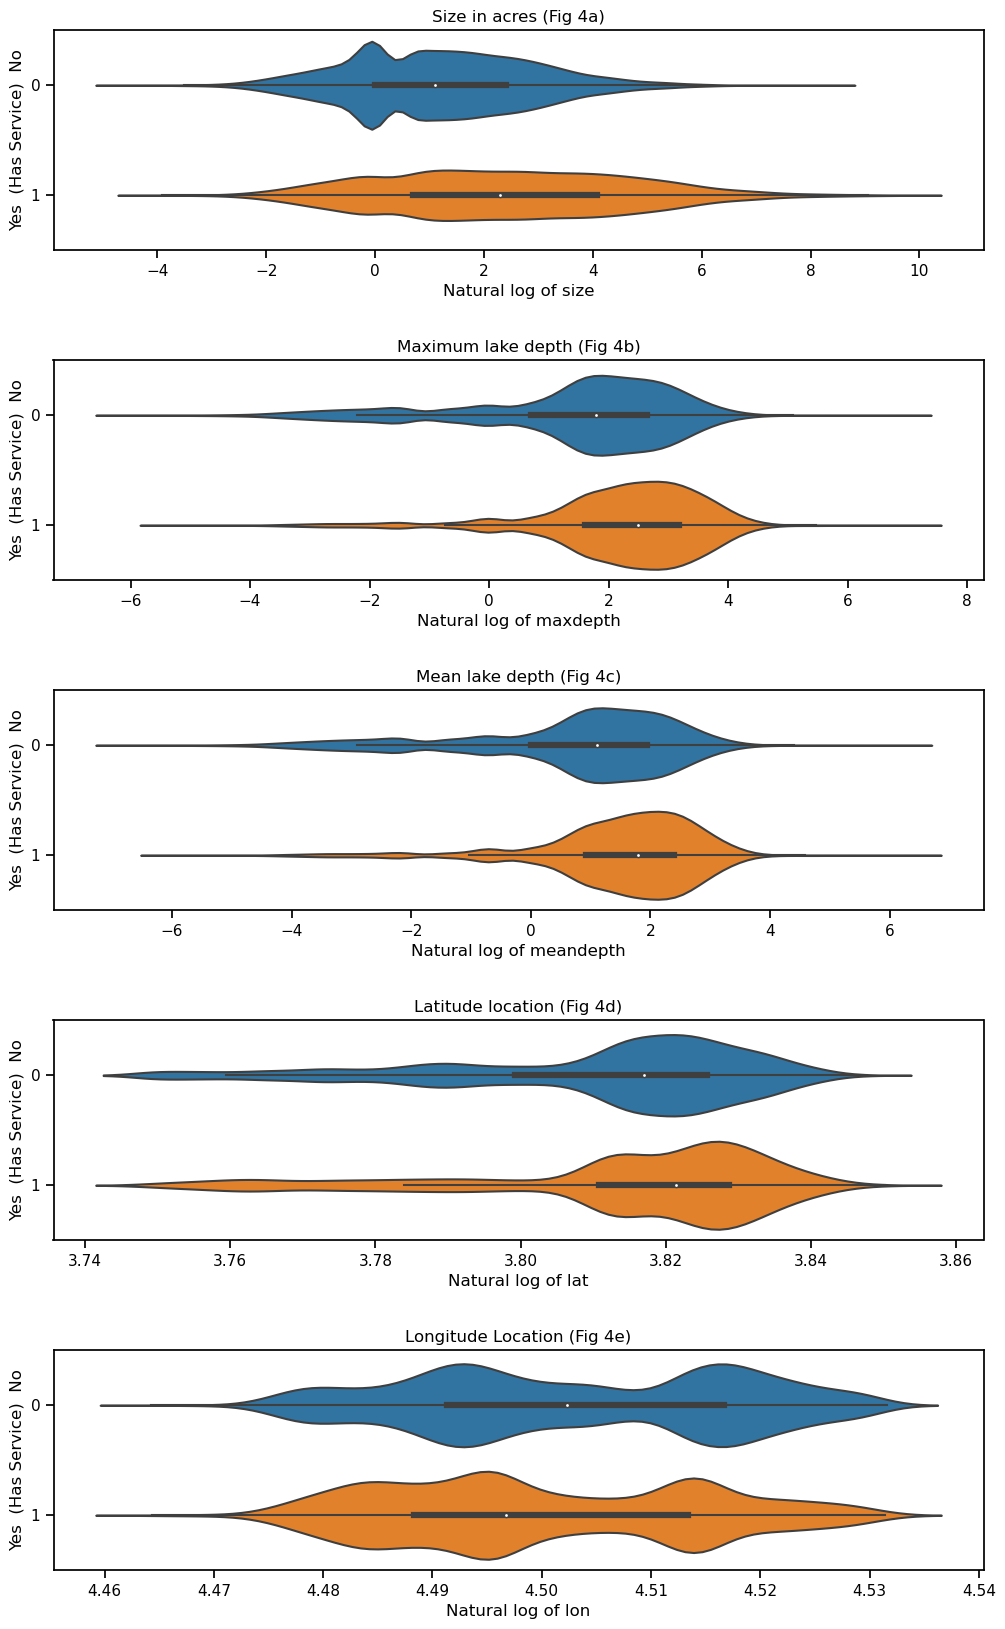
\includegraphics[keepaspectratio]{ParkSiteSelection_files/figure-pdf/fig-violin-plot-output-1.png}}

}

\caption{\label{fig-violin-plot}Violin plots exploring how the presence
of services differentiate by continuous variables from the WDNR data.}

\end{figure}%

Specifically lake size, maximum depth, and mean depth, the top three
plots in Figure~\ref{fig-violin-plot} show differences between lakes
that do and do not have public services. In each of these cases, lakes
with services (in orange) tend to be shifted to the right along the
x-axis, meaning they are generally larger and deeper than lakes without
services (in blue). Not only are the central tendencies higher for lakes
with services, but the spread of values is also wider, particularly for
size, suggesting a greater diversity in lake sizes among serviced lakes.
These differences imply that lake size and depth may be strong
predictors for whether a lake has public services.

On latitude and longitude, the bottom two plots of
Figure~\ref{fig-violin-plot}, show less pronounced differences. There is
modest separation in the distributions for lakes with and without
services, particularly in latitude, where lakes with public services
appear to be slightly more concentrated in certain geographic bands.
This may reflect regional planning priorities or population density
factors but likely provides less predictive value than physical lake
characteristics.

\begin{tcolorbox}[enhanced jigsaw, coltitle=black, toprule=.15mm, arc=.35mm, bottomtitle=1mm, opacityback=0, leftrule=.75mm, left=2mm, colframe=quarto-callout-note-color-frame, toptitle=1mm, titlerule=0mm, breakable, colbacktitle=quarto-callout-note-color!10!white, colback=white, bottomrule=.15mm, title=\textcolor{quarto-callout-note-color}{\faInfo}\hspace{0.5em}{Note}, rightrule=.15mm, opacitybacktitle=0.6]

The continuous variables displayed in Figure 4 have long-tailed,
highly-skewed distributions. To make the visualizations more
interpretable and to reduce the influence of extreme values, I applied
the natural logarithm transformation. This common transformation
compresses the scale of larger values. The result is a more readable
distribution.

\end{tcolorbox}

These visual explorations serve as an important visual check on the
potential predictive power of each feature when modeling the presence of
public service. The greater the separation between the two
distributions, the more likely that variable will be useful in a
classification task. Based on the WDNR data, features like size, max
depth, and mean depth appear to have strong potential as predictors,
while latitude and longitude may contribute some additional nuance when
combined with other variables.

One additional customary plot used in exploratory data anlysis is the
pair plot. Below Figure~\ref{fig-logpairplot_1} again reveals the same
patterns noted above in Table~\ref{tbl-prepared-summary} and
Figure~\ref{fig-violin-plot}.

\begin{Shaded}
\begin{Highlighting}[]
\CommentTok{\# Produce a filtered pairplot excluding observations that had missing max depth}
\NormalTok{log\_pairplot }\OperatorTok{=}\NormalTok{ sns.pairplot(}
\NormalTok{    df[(df[}\StringTok{\textquotesingle{}maxdepth\_missing\textquotesingle{}}\NormalTok{] }\OperatorTok{!=} \VariableTok{True}\NormalTok{) }\OperatorTok{\&}\NormalTok{ (df[}\StringTok{\textquotesingle{}meandepth\_missing\textquotesingle{}}\NormalTok{] }\OperatorTok{!=} \VariableTok{True}\NormalTok{)]}
\NormalTok{    [[}\StringTok{\textquotesingle{}size\textquotesingle{}}\NormalTok{,}\StringTok{\textquotesingle{}maxdepth\textquotesingle{}}\NormalTok{,}\StringTok{\textquotesingle{}meandepth\textquotesingle{}}\NormalTok{,}\StringTok{\textquotesingle{}hasservice\textquotesingle{}}\NormalTok{]],}
\NormalTok{    hue}\OperatorTok{=}\StringTok{\textquotesingle{}hasservice\textquotesingle{}}\NormalTok{, aspect}\OperatorTok{=}\DecValTok{2}\NormalTok{)}

\ControlFlowTok{for}\NormalTok{ ax }\KeywordTok{in}\NormalTok{ log\_pairplot.axes.flatten():  }\CommentTok{\# Iterate over all subplots}
\NormalTok{    ax.set\_xscale(}\StringTok{\textquotesingle{}log\textquotesingle{}}\NormalTok{)}
\NormalTok{    ax.set\_yscale(}\StringTok{\textquotesingle{}log\textquotesingle{}}\NormalTok{)}\OperatorTok{;}
\end{Highlighting}
\end{Shaded}

\begin{figure}[H]

\centering{

\pandocbounded{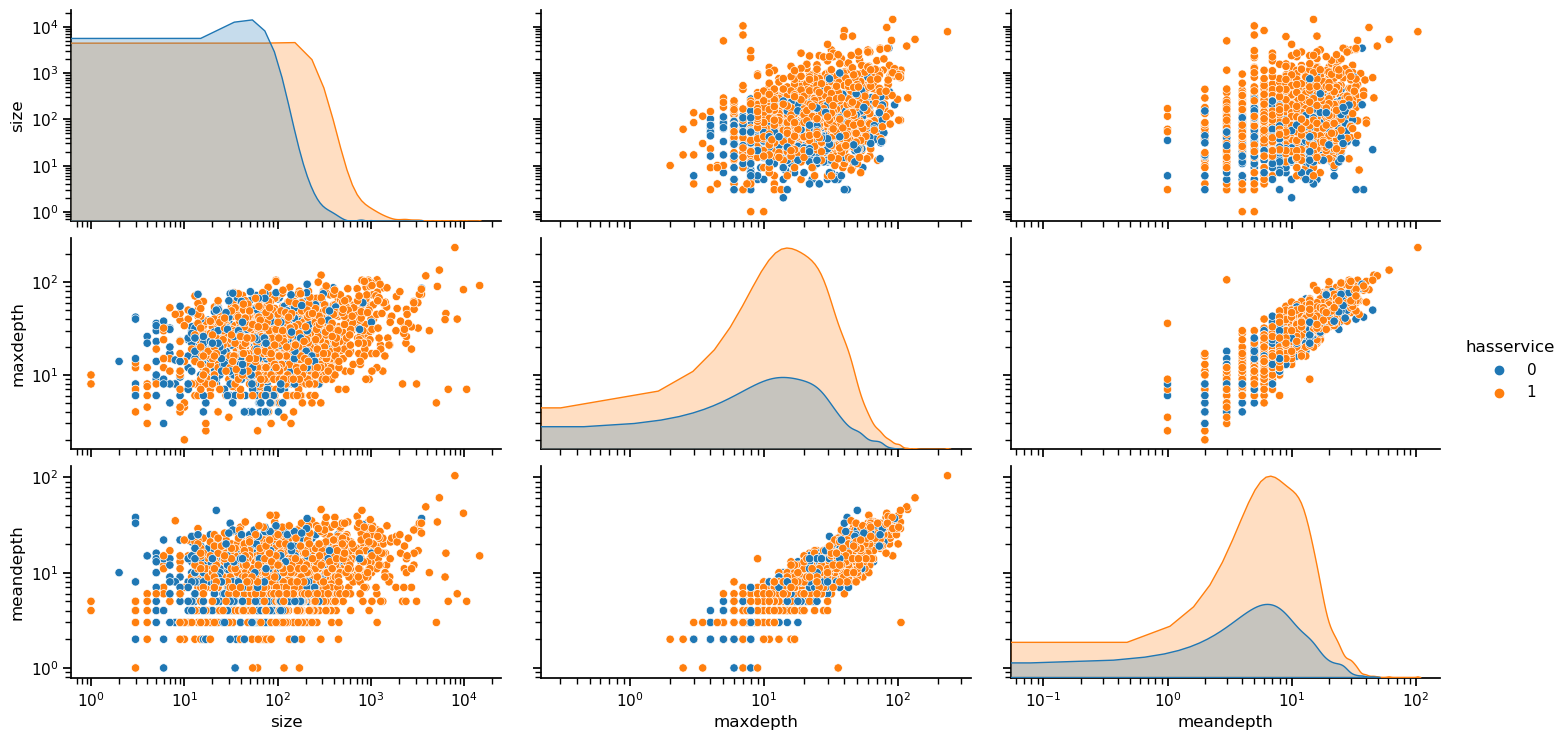
\includegraphics[keepaspectratio]{ParkSiteSelection_files/figure-pdf/fig-logpairplot_1-output-1.png}}

}

\caption{\label{fig-logpairplot_1}A Traditional Pairplot.}

\end{figure}%

\subsection{Binary Variable
Exploration}\label{binary-variable-exploration}

These WDNR data also consist of multiple columns of a binary nature,
reporting the presence of specific fish species including catfish,
largemouth bass, musky, northern pike, panfish, smallmouth bass,
sturgeon, trout, and walleye. Instead of exploring the potential
predictive value of these binary with violin plots we must turn to other
options such as chi square analysis which is well suited to test the
whether the presence of a publice service may be a function of the
presence of any given species.

\begin{Shaded}
\begin{Highlighting}[]
\CommentTok{\# List of binary fish species columns}
\NormalTok{fish\_cols }\OperatorTok{=}\NormalTok{ [}
    \StringTok{\textquotesingle{}Catfish\textquotesingle{}}\NormalTok{, }\StringTok{\textquotesingle{}Largemouth Bass\textquotesingle{}}\NormalTok{, }\StringTok{\textquotesingle{}Musky\textquotesingle{}}\NormalTok{,}
    \StringTok{\textquotesingle{}Northern Pike\textquotesingle{}}\NormalTok{, }\StringTok{\textquotesingle{}Panfish\textquotesingle{}}\NormalTok{, }\StringTok{\textquotesingle{}Smallmouth Bass\textquotesingle{}}\NormalTok{,}
    \StringTok{\textquotesingle{}Sturgeon\textquotesingle{}}\NormalTok{, }\StringTok{\textquotesingle{}Trout\textquotesingle{}}\NormalTok{, }\StringTok{\textquotesingle{}Walleye\textquotesingle{}}\NormalTok{]}

\CommentTok{\# Establish an empty results dictionary}
\NormalTok{chi2\_stats }\OperatorTok{=}\NormalTok{ \{\}}

\CommentTok{\# Loop through fish columns and compute Chi{-}square stat vs. hasservice}
\ControlFlowTok{for}\NormalTok{ col }\KeywordTok{in}\NormalTok{ fish\_cols:}
\NormalTok{    contingency\_table }\OperatorTok{=}\NormalTok{ pd.crosstab(df[col], df[}\StringTok{\textquotesingle{}hasservice\textquotesingle{}}\NormalTok{])}
\NormalTok{    chi2\_stat, p\_value, dof, expected }\OperatorTok{=}\NormalTok{ chi2\_contingency(contingency\_table)}
\NormalTok{    chi2\_stats[col] }\OperatorTok{=}\NormalTok{ [chi2\_stat, p\_value, dof, expected]}

\CommentTok{\# Initilize the beginning of a discussion}
\NormalTok{chi2\_summary }\OperatorTok{=} \StringTok{"All fish species columns appear to offer some predictive value. "}

\CommentTok{\# Generate and populate discussion with results from the analysis}
\ControlFlowTok{for}\NormalTok{ i, (species, stats) }\KeywordTok{in} \BuiltInTok{list}\NormalTok{(}\BuiltInTok{enumerate}\NormalTok{(chi2\_stats.items()))[:}\OperatorTok{{-}}\DecValTok{1}\NormalTok{]:}
    \CommentTok{\#print(f"\{species\}: χ² = \{stats[0]:.3f\} (p{-}value = \{stats[1]:.4f)")}
\NormalTok{    chi2\_summary }\OperatorTok{+=} \SpecialStringTok{f"""For }\SpecialCharTok{\{}\NormalTok{species}\SpecialCharTok{.}\NormalTok{lower()}\SpecialCharTok{\}}\SpecialStringTok{ we find the χ² value of }
\SpecialStringTok{        }\SpecialCharTok{\{}\NormalTok{stats[}\DecValTok{0}\NormalTok{]}\SpecialCharTok{:.3f\}}\SpecialStringTok{ (p{-}value = }\SpecialCharTok{\{}\NormalTok{stats[}\DecValTok{1}\NormalTok{]}\SpecialCharTok{:.4f\}}\SpecialStringTok{). """}

\CommentTok{\# Write the last entry of the iterative discussion}
\NormalTok{chi2\_summary }\OperatorTok{+=} \SpecialStringTok{f"""And finally for }\SpecialCharTok{\{}\NormalTok{species}\SpecialCharTok{\}}\SpecialStringTok{ we }
\SpecialStringTok{        find the we find the χ² value of }
\SpecialStringTok{        }\SpecialCharTok{\{}\NormalTok{stats[}\DecValTok{0}\NormalTok{]}\SpecialCharTok{:.3f\}}\SpecialStringTok{ (p{-}value = }\SpecialCharTok{\{}\NormalTok{stats[}\DecValTok{1}\NormalTok{]}\SpecialCharTok{:.4f\}}\SpecialStringTok{)."""}

\CommentTok{\# Display the discussion}
\NormalTok{display(Markdown(chi2\_summary))}
\end{Highlighting}
\end{Shaded}

All fish species columns appear to offer some predictive value. For
catfish we find the χ² value of 70.197 (p-value = 0.0000). For
largemouth bass we find the χ² value of 1370.317 (p-value = 0.0000). For
musky we find the χ² value of 579.412 (p-value = 0.0000). For northern
pike we find the χ² value of 1269.510 (p-value = 0.0000). For panfish we
find the χ² value of 1314.865 (p-value = 0.0000). For smallmouth bass we
find the χ² value of 504.343 (p-value = 0.0000). For sturgeon we find
the χ² value of 67.221 (p-value = 0.0000). For trout we find the χ²
value of 197.378 (p-value = 0.0000). And finally for Trout we find the
we find the χ² value of 197.378 (p-value = 0.0000).

\subsection{Machine Learning Predictions As
Recommendations}\label{machine-learning-predictions-as-recommendations}

James et al. (2023) explain that ``broadly speaking, supervised
statistical learning involves building a statistical model for
predicting, or estimating, an output based on one or more inputs''
(p.~1). Data science methods genreally aim to leverage a series of
features which can reliably predict an outcome.

In this paper's analysis the outcome is whether a lake has as public
service while the predictors are each lake's size in acers, maximum
depth, mean depth, latitude, longitude, type
(\textbf{?var:lake\_type\_vals}), clarity
(\textbf{?var:lake\_clarity\_vals}), and the presence of specific fish
species (\textbf{?var:fish\_species\_list}).

Through the use of a predictive algorithm that measures similarity this
paper's analysis will first create a model that looks to predict which
of Wisconsin's lakes have a public service and which of Wisconsin's
lakes do not have a public service. Inevitably there will be some
errors.

One set of errors will be lakes that do not have a service but that the
model predicted would (becauase they are similar to others that do)
which we will call overserviced. Likewise another set of errors will be
lakes that do have a service but that model predicted would not (becuase
these other lakes are more similar to those that do not have service)
which we will call underserviced.

\subsection{k-Nearest Neighbors (KNN)}\label{k-nearest-neighbors-knn}

To classify whether a lake should or should not have a public service,
this paper turns to a classic algorithm known as k-Nearest Neighbors
(KNN). More traditionally, this algorithm serves to predict class
membership based on an observation's similarity to other observations of
a known classification.

KNN is a non-parametric, instance-based learning algorithm that does not
make assumptions about the underlying distribution of the data. Instead,
it classifies instances based on the majority class of their closest
neighbors in a feature space. Which is a technical manner of explaining
that KNN is a way for a computer algorithm to make predictions or
conclusions about an object based on what it ``sees'' (or measures using
euclidian distances) as other similar objects.

A simplified version of the KNN process, as it operates for this paper,
is to first observe an unknown lake and its characteristic features.
Suppose the unknown lake is less than one acre in surface area and also
less than 6 feet deep at its max. Then further suppose that 99\% of all
lakes less than an acre in size and also around 6 feet deep (+/- one
foot) have no public service. Thus it would appear that the unknown lake
is similar to lakes with no service and accordingly the algorithm would
predict the uknown lake as one that also would have no public services.

In data science we use the term \emph{non-parametric} to describe
predictive algorithms, such as KNN, which have no fixed formula. Being
absent a fixed formula distinguishes the non-parametic approach from
parametric approaches, such as logistic regression, for example. James
et al. (2023) describe KNN as one of ``the simplest and best-known
non-parametric methods'' (p.~111).

Models that are \emph{instance-based} make decisions by comparing one
instance (or given this paper's data any instance of a given lake) to
others instances (other lakes). During the model fit procedure the
algorithm memorizes the training data by storing as a reference all
training instances. A \emph{feature space} is a term for the way we
describe the multi-dimensional, or multi-variate, nature of the
predictive features and their values.

\begin{tcolorbox}[enhanced jigsaw, coltitle=black, toprule=.15mm, arc=.35mm, bottomtitle=1mm, opacityback=0, leftrule=.75mm, left=2mm, colframe=quarto-callout-note-color-frame, toptitle=1mm, titlerule=0mm, breakable, colbacktitle=quarto-callout-note-color!10!white, colback=white, bottomrule=.15mm, title=\textcolor{quarto-callout-note-color}{\faInfo}\hspace{0.5em}{Note}, rightrule=.15mm, opacitybacktitle=0.6]

This distance metric must not be conflated for geographic distance. For
example, two lakes located on opposite sides of the state may still be
considered ``close'' in feature space if they share similar size, depth,
water clarity, and fish populations. This abstract notion of distance
allows KNN to make predictions based on overall similarity in
characteristics, rather than geographic location alone.

\end{tcolorbox}

In this paper's data, the feature space includes dimensions such as lake
size, maximum depth, mean depth, latitude, longitude, water clarity, and
the presence of specific fish species. The KNN algorithm uses this
feature space to calculate distances between lakes and identify their
nearest neighbors, which helps classify them based on their similarity.

\section{Analysis}\label{analysis}

This analysis uses the open-source Python package Scikit-learn
(https://scikit-learn.org), a widely adopted and well-documented
framework for implementing machine learning models, including k-nearest
neighbors (KNN). Scikit-learn supports reproducible and transparent
research, making it ideal for applications in data science and policy
evaluation.

\textbf{TODO: Add Sklearn documenation as a source.}

The analytical procedures in this paper align with those outlined in
Chapter 11 of Nelson (2023) and Chapter 3 of Raschka and Mirjalili
(2019). Most machine learning workflows begin by splitting the available
data into training and testing sets. The training set allows the model
to learn patterns and relationships in the data, while the testing set
remains untouched until final evaluation. This split helps ensure that
performance estimates reflect how the model will generalize to new data
not seen during training.

The training and testing sets also support model parameter selection. In
this case the parameter to optimize is the optimal number of \emph{k}
neighbors in the KNN algorithm. As is also customary, to avoid
information leakage, this analysis performs data preprocessing after the
data has been split. Binary features (such as fish species presence)
require no further transformation. However, nominal features such as
clarity and type are converted into dummy variables using one-hot
encoding, and all continuous predictors are rescaled using a
standardization procedure to ensure they contribute equally to distance
calculations.

Following transformation, the next step involves conducting a parameter
search to identify the most effective value for \emph{k}, the number of
nearest neighbors used in the KNN algorithm. In most cases, the
customary approach is to select the smallest value of \emph{k} that also
minimizes prediction error. A smaller \emph{k} yields a simpler, more
interpretable model. However, this paper intentionally selects a
less-well performing k value to relize a more complex model. The
reasoning behind this choice is practical: a more complex model yields a
finer-grained and more complete distribution of predicted probabilities.
These probabilities in turn, support a more nuanced analysis of false
predictions. As the anslysis seeks to identify lakes that do not have
public services but appear similar to those that do, and vice versa.
This added granularity enhances the utility of the model in producing
actionable policy recommendations.

As a final step, this analysis uses a two-fold cross-validation with
symmetric evaluation, which ensures that every lake is evaluated as an
out-of-sample observation exactly once. In the first fold, the model is
trained on half of the data and used to predict outcomes for the other
half; in the second fold, the roles are reversed. This method yields a
complete set of out-of-sample predictions, which allows us to identify
false positives (lakes without public services that resemble lakes that
do) and false negatives (lakes with public services that resemble those
that don't). These classification errors serve as the empirical
foundation for the policy recommendations presented later in this paper.

\subsection{Train Test Split
Procedure}\label{train-test-split-procedure}

The SciKit Learn user guide states plainly that ``Learning the
parameters of a prediction function and testing it on the same data is a
methodological mistake'' Scikit-Learn (2023). This mistake would usually
lead to a model that has \emph{overfit}. Instead of finding the general
functional relationships between predictor features and an outcome, a
model that has overfit to the data, has come close to memorizing the
training data.

By first fitting a model on a subset of training data and then using a
separate hold out subset as a test, the procedure results in a more
objective opportunity to fairly evaluate the predictive abilities of a
model. The procedure ensures that a model which performs well on
training data also later performs well on new data yet to be generated
in future production settings.

\begin{Shaded}
\begin{Highlighting}[]
\CommentTok{\# Organize Features + Predictors}
\NormalTok{ready\_features }\OperatorTok{=}\NormalTok{ [}
    \StringTok{\textquotesingle{}Catfish\textquotesingle{}}\NormalTok{,}\StringTok{\textquotesingle{}Largemouth Bass\textquotesingle{}}\NormalTok{, }\StringTok{\textquotesingle{}Musky\textquotesingle{}}\NormalTok{, }\StringTok{\textquotesingle{}Northern Pike\textquotesingle{}}\NormalTok{, }
    \StringTok{\textquotesingle{}Panfish\textquotesingle{}}\NormalTok{, }\StringTok{\textquotesingle{}Smallmouth Bass\textquotesingle{}}\NormalTok{, }\StringTok{\textquotesingle{}Sturgeon\textquotesingle{}}\NormalTok{, }\StringTok{\textquotesingle{}Trout\textquotesingle{}}\NormalTok{, }\StringTok{\textquotesingle{}Walleye\textquotesingle{}}\NormalTok{]}
\NormalTok{con\_features }\OperatorTok{=}\NormalTok{ [}\StringTok{\textquotesingle{}size\textquotesingle{}}\NormalTok{,}\StringTok{\textquotesingle{}maxdepth\textquotesingle{}}\NormalTok{, }\StringTok{\textquotesingle{}meandepth\textquotesingle{}}\NormalTok{, }\StringTok{\textquotesingle{}lat\textquotesingle{}}\NormalTok{, }\StringTok{\textquotesingle{}lon\textquotesingle{}}\NormalTok{]}
\NormalTok{bin\_features }\OperatorTok{=}\NormalTok{ [}\StringTok{\textquotesingle{}maxdepth\_missing\textquotesingle{}}\NormalTok{, }\StringTok{\textquotesingle{}meandepth\_missing\textquotesingle{}}\NormalTok{]}
\NormalTok{cat\_features }\OperatorTok{=}\NormalTok{ [}\StringTok{\textquotesingle{}type\textquotesingle{}}\NormalTok{, }\StringTok{\textquotesingle{}clarity\textquotesingle{}}\NormalTok{]}

\CommentTok{\# Establish X (predictor) and y (target) matricies}
\NormalTok{X }\OperatorTok{=}\NormalTok{ df[con\_features }\OperatorTok{+}\NormalTok{ bin\_features }\OperatorTok{+}\NormalTok{ ready\_features }\OperatorTok{+}\NormalTok{ cat\_features]}
\NormalTok{y }\OperatorTok{=}\NormalTok{ df[}\StringTok{\textquotesingle{}hasservice\textquotesingle{}}\NormalTok{]}

\CommentTok{\# Perform train test split with SkLearn}
\NormalTok{X\_train, X\_test, y\_train, y\_test }\OperatorTok{=}\NormalTok{ train\_test\_split(}
\NormalTok{    X, y, test\_size}\OperatorTok{=}\FloatTok{0.30}\NormalTok{, random\_state}\OperatorTok{=}\DecValTok{42}\NormalTok{, stratify}\OperatorTok{=}\NormalTok{y)}
\end{Highlighting}
\end{Shaded}

\subsection{Rescale Continuous Data}\label{rescale-continuous-data}

According to Raschka and Mirjalili (2019) ``the majority of machine
learning\ldots{} algorithms behave much better if features are on the
same scale'' (p.~124). In the case of KNN, an algorithm that relies on
calculating distances between data points in the feature space, if the
features spread across vastly different scales, those with larger ranges
will dominate the distance calculations.

Fitting a KNN on features that are differently scaled may potentially
lead to biased classifications. For instance, if one feature represents
lake size in acres (ranging from tens to thousands) and another
represents water clarity on a scale of 1 to 100, the size feature will
disproportionately influence the nearest neighbor determination. Thus,
For KNN, rescaling ensures that all features contribute equally to the
distance metric (Nelson 2023, 317).

To address this issue, continuous data is typically rescaled to 0 to 1,
-1 to 1, or to z-score values which places the mean at 0 and then shifts
values so there is a standard deviation of 1. In this paper I proceed
with a 0 to 1 scale.

\begin{Shaded}
\begin{Highlighting}[]
\NormalTok{scaler }\OperatorTok{=}\NormalTok{ StandardScaler()}
\NormalTok{ohe }\OperatorTok{=}\NormalTok{ OneHotEncoder(sparse\_output}\OperatorTok{=}\VariableTok{False}\NormalTok{, }
\NormalTok{                    handle\_unknown}\OperatorTok{=}\StringTok{\textquotesingle{}ignore\textquotesingle{}}\NormalTok{).set\_output(transform}\OperatorTok{=}\StringTok{\textquotesingle{}pandas\textquotesingle{}}\NormalTok{)}

\CommentTok{\# Rescale continuous variables}
\NormalTok{X\_train[con\_features] }\OperatorTok{=}\NormalTok{ scaler.fit\_transform(X\_train[con\_features])}
\NormalTok{X\_test[con\_features] }\OperatorTok{=}\NormalTok{ scaler.transform(X\_test[con\_features])}

\CommentTok{\# One hot encode nominal categorical}
\NormalTok{X\_train\_ohe }\OperatorTok{=}\NormalTok{ ohe.fit\_transform(X\_train[cat\_features])}
\NormalTok{X\_test\_ohe }\OperatorTok{=}\NormalTok{ ohe.transform(X\_test[cat\_features])}

\CommentTok{\# Drop original categorical cols and concat OHE output}
\NormalTok{X\_train }\OperatorTok{=}\NormalTok{ pd.concat([X\_train.drop(cat\_features, axis}\OperatorTok{=}\DecValTok{1}\NormalTok{), X\_train\_ohe], axis}\OperatorTok{=}\DecValTok{1}\NormalTok{)}
\NormalTok{X\_test }\OperatorTok{=}\NormalTok{ pd.concat([X\_test.drop(cat\_features, axis}\OperatorTok{=}\DecValTok{1}\NormalTok{), X\_test\_ohe], axis}\OperatorTok{=}\DecValTok{1}\NormalTok{)}
\end{Highlighting}
\end{Shaded}

\subsection{Fit Base Model}\label{fit-base-model}

Before proceeding with parameter tuning or model refinement, it is often
useful to fit a base model using an arbitrary but reasonable choice of
parameters. In the case of k-nearest neighbors (KNN), selecting a base
\emph{k} such as \emph{k} = 19. This base model provides an initial
benchmark for model performance. This step, though technically optional,
serves several important purposes within the broader analytical process.

First, fitting a base model allows the analyst to ensure that the
pipeline---from data preprocessing to model training and evaluation
functioned as intended. Errors related to data structure, scaling,
encoding, or other preprocessing steps often surface during this
preliminary fit. The base model thus acts as a diagnostic opportunity to
detect problems before introducing additional complexity through
cross-validation, parameter searches, or other hyperparameter tuning
efforts.

Second, the base model offers a reference point for evaluating the value
added by subsequent modeling decisions. For example, if the accuracy or
error rate of a tuned model differs only marginally from that of the
base model, the analyst may reconsider the complexity or
interpretability trade-offs involved in optimization. Conversely, large
improvements over the base model suggest meaningful gains that justify
further refinement.

Finally, the base model supports replication and transparency by
providing a fixed and reproducible result that others can use to
validate or extend the work. By producing and recording model
performance with arbitrary but documented parameters, the analysis
builds a foundation upon which subsequent results can be compared,
especially in applied contexts where interpretability and policy
implications matter as much as technical performance.

In short, while fitting a base model with arbitrary \emph{k} is not
strictly necessary for most analyses, it offers extensive practical
value in building a rigorous, transparent, and well-structured analysis.

\begin{Shaded}
\begin{Highlighting}[]
\CommentTok{\# Instantiate a base model with 19 neighbors}
\NormalTok{knn\_base }\OperatorTok{=}\NormalTok{ KNeighborsClassifier(n\_neighbors}\OperatorTok{=}\DecValTok{19}\NormalTok{)}

\CommentTok{\# Fit the model using training data}
\NormalTok{knn\_base.fit(X\_train, y\_train)}
\NormalTok{y\_pred }\OperatorTok{=}\NormalTok{ knn\_base.predict(X\_test)}
\end{Highlighting}
\end{Shaded}

This base model yeild \textbf{?var:base\_accuracy} accuracy (correct
classifications). There were \textbf{?var:base\_false\_pos} false
positive predictions and \textbf{?var:base\_false\_neg} false negative
predictions. These base metrics can serve as a helpful reference when
evaluating futher results below.

\subsection{Evaluate + Search for Optimal
K}\label{evaluate-search-for-optimal-k}

This portion of the analysis implements a parameter search to determine
how the choice of \emph{k} (the number of neighbors considered in the
KNN classification algorithm) affects model performance. The goal is to
identify a value of \emph{k} that yields relatively low classification
error, thereby improving the model's predictive accuracy. As discussed
above, for this paper I will not choose the lowest error rate in order
to support a fully nuanced analysis.

This portion of the analysis begins by initializing an empty list named
\texttt{error\_rates} to store the error rate associated with each value
of \emph{k}. The \texttt{for} loop then iterates through odd-numbered
values of \emph{k} from 1 to 99. Odd values avoid tie votes in binary
classification. For each iteration, the code instantiates a new
\texttt{KNeighborsClassifier} model using the current value of \emph{k}
and fits it to the training data.

Once trained the code predicts classifications for the testing set
(\texttt{X\_test}), then calculates the error rate as the proportion of
incorrect predictions, and appends that result to the
\texttt{error\_rates} list. By the end of the loop, the list holds the
model's error rates across a range of \emph{k} values.

\begin{Shaded}
\begin{Highlighting}[]
\CommentTok{\# Instantiate an empty list of errors}
\NormalTok{error\_rates }\OperatorTok{=}\NormalTok{ []}

\CommentTok{\# Iterate through odd numbered neighbors 1 through 99}
\ControlFlowTok{for}\NormalTok{ k }\KeywordTok{in} \BuiltInTok{range}\NormalTok{(}\DecValTok{1}\NormalTok{, }\DecValTok{100}\NormalTok{, }\DecValTok{2}\NormalTok{):}
    \CommentTok{\# The KNN classification model}
\NormalTok{    knn }\OperatorTok{=}\NormalTok{ KNeighborsClassifier(n\_neighbors}\OperatorTok{=}\NormalTok{k)}
\NormalTok{    knn.fit(X\_train, y\_train)}
    
    \CommentTok{\# Generate predictions on the testing data}
\NormalTok{    y\_pred\_kn }\OperatorTok{=}\NormalTok{ knn.predict(X\_test)}
    
    \CommentTok{\# Calculate and record proprtion of correct classifications}
\NormalTok{    error\_rates.append(np.mean(y\_pred\_kn }\OperatorTok{!=}\NormalTok{ y\_test))}
\end{Highlighting}
\end{Shaded}

A subsequent block of code generates Figure~\ref{fig-error_rates}, a
visual representation of the results using Matplotlib.
Figure~\ref{fig-error_rates} uses a dotted blue line with `x' markers to
show how error rates change as \emph{k} increases.

By examining Figure~\ref{fig-error_rates}'s curve, an analyst can make
an informed decision about which \emph{k} values to consider for the
final model---balancing error rate, model simplicity, and practical
interpretability. Given these results I choose a \emph{k} value of 29
consistent with the procedure outlined above.

\begin{Shaded}
\begin{Highlighting}[]
\CommentTok{\# Visualize the results of the search above}
\NormalTok{plt.figure(figsize}\OperatorTok{=}\NormalTok{(}\DecValTok{8}\NormalTok{, }\DecValTok{4}\NormalTok{))           }\CommentTok{\# Landscape Sizing}

\CommentTok{\# Match plot range to for loop above {-} add style for readability}
\NormalTok{plt.plot(}\BuiltInTok{range}\NormalTok{(}\DecValTok{1}\NormalTok{, }\DecValTok{100}\NormalTok{, }\DecValTok{2}\NormalTok{), error\_rates, color}\OperatorTok{=}\StringTok{\textquotesingle{}blue\textquotesingle{}}\NormalTok{,}
\NormalTok{         linestyle}\OperatorTok{=}\StringTok{\textquotesingle{}:\textquotesingle{}}\NormalTok{, marker}\OperatorTok{=}\StringTok{\textquotesingle{}x\textquotesingle{}}\NormalTok{, markersize}\OperatorTok{=}\DecValTok{5}\NormalTok{)}

\NormalTok{plt.annotate(text}\OperatorTok{=}\StringTok{\textquotesingle{}Chosen K (29)\textquotesingle{}}\NormalTok{, }
\NormalTok{             xy}\OperatorTok{=}\NormalTok{(}\DecValTok{30}\NormalTok{, }\FloatTok{.233}\NormalTok{), xytext}\OperatorTok{=}\NormalTok{(}\DecValTok{50}\NormalTok{, }\FloatTok{.237}\NormalTok{), fontsize}\OperatorTok{=}\DecValTok{10}\NormalTok{,}
\NormalTok{             arrowprops}\OperatorTok{=}\NormalTok{\{}\StringTok{\textquotesingle{}arrowstyle\textquotesingle{}}\NormalTok{:}\StringTok{\textquotesingle{}{-}\textgreater{}\textquotesingle{}}\NormalTok{, }\StringTok{\textquotesingle{}connectionstyle\textquotesingle{}}\NormalTok{:}\StringTok{\textquotesingle{}arc3, rad={-}.2\textquotesingle{}}\NormalTok{\})}

\NormalTok{plt.title(}\StringTok{\textquotesingle{}Error vs. K Values\textquotesingle{}}\NormalTok{)      }\CommentTok{\# Chart Title}
\NormalTok{plt.xlabel(}\StringTok{\textquotesingle{}K Value\textquotesingle{}}\NormalTok{)                }\CommentTok{\# X Axis Title}
\NormalTok{plt.ylabel(}\StringTok{\textquotesingle{}Error Rate\textquotesingle{}}\NormalTok{)             }\CommentTok{\# Y Axis Title}
\end{Highlighting}
\end{Shaded}

\begin{figure}[H]

\centering{

\centering{

\begin{verbatim}
Text(0, 0.5, 'Error Rate')
\end{verbatim}

}

\subcaption{\label{fig-error_rates-1}A plot showing error rate over a
range of k values.}

\centering{

\pandocbounded{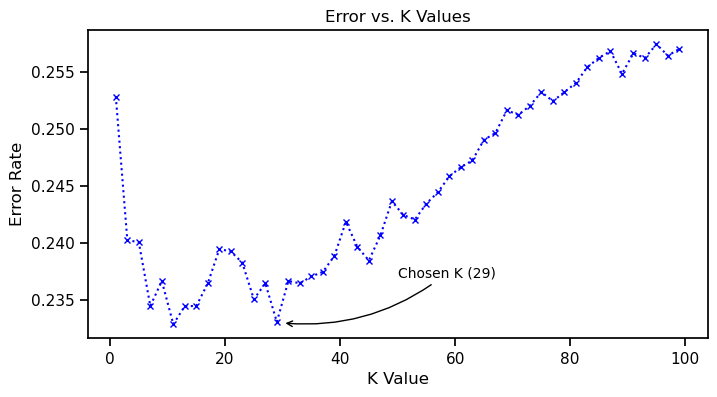
\includegraphics[keepaspectratio]{ParkSiteSelection_files/figure-pdf/fig-error_rates-output-2.png}}

}

\subcaption{\label{fig-error_rates-2}}

}

\caption{\label{fig-error_rates}}

\end{figure}%

\subsection{Two-fold cross-validation; Symmetric
evaluation}\label{two-fold-cross-validation-symmetric-evaluation}

In executing this procedure I first split the data into two equal
halves. In the first fold, I train the model on the first half and
predict on the second; in the second fold, the I reverse the process.

As before, within each fold, continuous variables are standardized using
\texttt{StandardScaler} and nominal categorical variables are
transformed via one-hot encoding using \texttt{OneHotEncoder}.

After each fit, train, and predict I record both the prediction and also
the probability of membership in the \texttt{hasservice} class. Finally,
I combine predictions from both folds and merged them back into the
original data. The result is a full set of out-of-sample predictions and
prediction probabilities for each observation.

\begin{Shaded}
\begin{Highlighting}[]
\CommentTok{\# Establish X (predictor) and y (target) matricies}
\NormalTok{X }\OperatorTok{=}\NormalTok{ df[con\_features }\OperatorTok{+}\NormalTok{ bin\_features }\OperatorTok{+}\NormalTok{ ready\_features }\OperatorTok{+}\NormalTok{ cat\_features]}
\NormalTok{y }\OperatorTok{=}\NormalTok{ df[}\StringTok{\textquotesingle{}hasservice\textquotesingle{}}\NormalTok{]}

\CommentTok{\# \# Perform initial 50/50 split}
\NormalTok{X\_A, X\_B, y\_A, y\_B }\OperatorTok{=}\NormalTok{ train\_test\_split(}
\NormalTok{    X, y, test\_size}\OperatorTok{=}\FloatTok{0.5}\NormalTok{, random\_state}\OperatorTok{=}\DecValTok{42}\NormalTok{, stratify}\OperatorTok{=}\NormalTok{y)}

\KeywordTok{def}\NormalTok{ execute\_fold(X\_train, X\_test, y\_train, y\_test):}
\NormalTok{    scaler }\OperatorTok{=}\NormalTok{ StandardScaler()}
\NormalTok{    ohe }\OperatorTok{=}\NormalTok{ OneHotEncoder(sparse\_output}\OperatorTok{=}\VariableTok{False}\NormalTok{, }
\NormalTok{                        handle\_unknown}\OperatorTok{=}\StringTok{\textquotesingle{}ignore\textquotesingle{}}\NormalTok{).set\_output(transform}\OperatorTok{=}\StringTok{\textquotesingle{}pandas\textquotesingle{}}\NormalTok{)}

    \CommentTok{\# Rescale continuous variables}
\NormalTok{    X\_train[con\_features] }\OperatorTok{=}\NormalTok{ scaler.fit\_transform(X\_train[con\_features])}
\NormalTok{    X\_test[con\_features] }\OperatorTok{=}\NormalTok{ scaler.transform(X\_test[con\_features])}

    \CommentTok{\# One hot encode nominal categorical}
\NormalTok{    X\_train\_ohe }\OperatorTok{=}\NormalTok{ ohe.fit\_transform(X\_train[cat\_features])}
\NormalTok{    X\_test\_ohe }\OperatorTok{=}\NormalTok{ ohe.transform(X\_test[cat\_features])}

    \CommentTok{\# Drop original categorical cols and concat OHE output}
\NormalTok{    X\_train }\OperatorTok{=}\NormalTok{ pd.concat([X\_train.drop(cat\_features, axis}\OperatorTok{=}\DecValTok{1}\NormalTok{), X\_train\_ohe], axis}\OperatorTok{=}\DecValTok{1}\NormalTok{)}
\NormalTok{    X\_test }\OperatorTok{=}\NormalTok{ pd.concat([X\_test.drop(cat\_features, axis}\OperatorTok{=}\DecValTok{1}\NormalTok{), X\_test\_ohe], axis}\OperatorTok{=}\DecValTok{1}\NormalTok{)}
    
    \CommentTok{\# Instantiate KNN Model}
\NormalTok{    knn\_cross }\OperatorTok{=}\NormalTok{ KNeighborsClassifier(n\_neighbors}\OperatorTok{=}\DecValTok{29}\NormalTok{)}

    \CommentTok{\# Fit the model using training data}
\NormalTok{    knn\_cross.fit(X\_train, y\_train)}
    \ControlFlowTok{return}\NormalTok{ pd.DataFrame(\{}
        \StringTok{\textquotesingle{}predicted\textquotesingle{}}\NormalTok{: knn\_cross.predict(X\_test),}
        \StringTok{\textquotesingle{}probability\textquotesingle{}}\NormalTok{: knn\_cross.predict\_proba(X\_test)[: ,}\DecValTok{1}\NormalTok{]\},}
\NormalTok{        index}\OperatorTok{=}\NormalTok{X\_test.index)}

\CommentTok{\# Train on A, predict on B}
\NormalTok{y\_B\_pred }\OperatorTok{=}\NormalTok{ execute\_fold(X\_A, X\_B, y\_A, y\_B)}

\CommentTok{\# Train on B, predict on A}
\NormalTok{y\_A\_pred }\OperatorTok{=}\NormalTok{ execute\_fold(X\_B, X\_A, y\_B, y\_A)}

\CommentTok{\# Stack the predictions}
\NormalTok{y\_preds }\OperatorTok{=}\NormalTok{ pd.concat([y\_B\_pred, y\_A\_pred])}

\CommentTok{\# Recompile the full data set}
\NormalTok{output\_cols }\OperatorTok{=}\NormalTok{ [}\StringTok{\textquotesingle{}ID\textquotesingle{}}\NormalTok{, }\StringTok{\textquotesingle{}name\textquotesingle{}}\NormalTok{, }\StringTok{\textquotesingle{}size\textquotesingle{}}\NormalTok{, }\StringTok{\textquotesingle{}maxdepth\textquotesingle{}}\NormalTok{, }\StringTok{\textquotesingle{}meandepth\textquotesingle{}}\NormalTok{, }
       \StringTok{\textquotesingle{}lat\textquotesingle{}}\NormalTok{, }\StringTok{\textquotesingle{}lon\textquotesingle{}}\NormalTok{, }\StringTok{\textquotesingle{}hasservice\textquotesingle{}}\NormalTok{, }\StringTok{\textquotesingle{}haslanding\textquotesingle{}}\NormalTok{, }\StringTok{\textquotesingle{}hasbeach\textquotesingle{}}\NormalTok{, }
       \StringTok{\textquotesingle{}haspark\textquotesingle{}}\NormalTok{, }\StringTok{\textquotesingle{}type\textquotesingle{}}\NormalTok{, }\StringTok{\textquotesingle{}clarity\textquotesingle{}}\NormalTok{, }\StringTok{\textquotesingle{}county\textquotesingle{}}\NormalTok{]}

\NormalTok{output\_data }\OperatorTok{=}\NormalTok{ df[output\_cols].copy()}

\NormalTok{output\_data }\OperatorTok{=}\NormalTok{ output\_data.merge(}
\NormalTok{    y\_preds, left\_index}\OperatorTok{=}\VariableTok{True}\NormalTok{, right\_index}\OperatorTok{=}\VariableTok{True}\NormalTok{, }
\NormalTok{    validate}\OperatorTok{=}\StringTok{\textquotesingle{}one\_to\_one\textquotesingle{}}\NormalTok{)}

\CommentTok{\# Save output\_data to csv}
\NormalTok{output\_data.to\_csv(}\StringTok{\textquotesingle{}output\_data.csv\textquotesingle{}}\NormalTok{, index}\OperatorTok{=}\VariableTok{True}\NormalTok{)}
\end{Highlighting}
\end{Shaded}

\section{Results}\label{results}

This analysis produced \textbf{?var:false\_preds\_count} false
predictions. A full list of all the lakes analyzed in this study and the
predictive results accompanies this project in a file called
\texttt{output\_data.csv}.

\begin{Shaded}
\begin{Highlighting}[]
\CommentTok{\# Summarise results, count false predictions}
\NormalTok{false\_preds\_count }\OperatorTok{=} \BuiltInTok{sum}\NormalTok{(output\_data[}\StringTok{\textquotesingle{}hasservice\textquotesingle{}}\NormalTok{] }\OperatorTok{!=}\NormalTok{ output\_data[}\StringTok{\textquotesingle{}predicted\textquotesingle{}}\NormalTok{])}

\CommentTok{\# Filter for false positives}
\NormalTok{false\_positives }\OperatorTok{=}\NormalTok{ output\_data[}
\NormalTok{    (output\_data[}\StringTok{\textquotesingle{}hasservice\textquotesingle{}}\NormalTok{] }\OperatorTok{==} \DecValTok{0}\NormalTok{) }\OperatorTok{\&} 
\NormalTok{    (output\_data[}\StringTok{\textquotesingle{}predicted\textquotesingle{}}\NormalTok{] }\OperatorTok{==} \DecValTok{1}\NormalTok{)]}

\CommentTok{\# Save count of false positives}
\NormalTok{false\_positive\_count }\OperatorTok{=}\NormalTok{ false\_positives.shape[}\DecValTok{0}\NormalTok{]}

\CommentTok{\# Filter for false negatives}
\NormalTok{false\_negatives }\OperatorTok{=}\NormalTok{ output\_data[}
\NormalTok{    (output\_data[}\StringTok{\textquotesingle{}hasservice\textquotesingle{}}\NormalTok{] }\OperatorTok{==} \DecValTok{1}\NormalTok{) }\OperatorTok{\&} 
\NormalTok{    (output\_data[}\StringTok{\textquotesingle{}predicted\textquotesingle{}}\NormalTok{] }\OperatorTok{==} \DecValTok{0}\NormalTok{)]}

\CommentTok{\# Save count of false negatives}
\NormalTok{false\_negative\_count }\OperatorTok{=}\NormalTok{ false\_negatives.shape[}\DecValTok{0}\NormalTok{]}

\CommentTok{\# Save these data for later reference}
\ControlFlowTok{with} \BuiltInTok{open}\NormalTok{(}\StringTok{"\_variables.yml"}\NormalTok{, }\StringTok{"a"}\NormalTok{) }\ImportTok{as}\NormalTok{ f:}
\NormalTok{    f.write(}\SpecialStringTok{f"false\_preds\_count: }\SpecialCharTok{\{}\NormalTok{false\_preds\_count}\SpecialCharTok{\}}\CharTok{\textbackslash{}n}\SpecialStringTok{"}\NormalTok{)}
\NormalTok{    f.write(}\SpecialStringTok{f"false\_positive\_count: }\SpecialCharTok{\{}\NormalTok{false\_positive\_count}\SpecialCharTok{\}}\CharTok{\textbackslash{}n}\SpecialStringTok{"}\NormalTok{)}
\NormalTok{    f.write(}\SpecialStringTok{f"false\_negative\_count: }\SpecialCharTok{\{}\NormalTok{false\_negative\_count}\SpecialCharTok{\}}\CharTok{\textbackslash{}n}\SpecialStringTok{"}\NormalTok{)}
\end{Highlighting}
\end{Shaded}

\begin{Shaded}
\begin{Highlighting}[]
\CommentTok{\# Initiate paragraph describing false positive results}
\NormalTok{false\_pos\_desc }\OperatorTok{=} \SpecialStringTok{f"Overall there were }\SpecialCharTok{\{}\NormalTok{false\_positive\_count}\SpecialCharTok{\}}\SpecialStringTok{ false positives. "}
\NormalTok{false\_pos\_desc }\OperatorTok{+=} \StringTok{"Among the false positives there were "}

\CommentTok{\# Write paragraph describing false positive results}
\ControlFlowTok{for}\NormalTok{ p, lcount }\KeywordTok{in} \BuiltInTok{list}\NormalTok{(}
\NormalTok{    false\_positives[}\StringTok{\textquotesingle{}probability\textquotesingle{}}\NormalTok{].value\_counts().sort\_index().to\_dict().items())[:}\OperatorTok{{-}}\DecValTok{1}\NormalTok{]:}
\NormalTok{    false\_pos\_desc }\OperatorTok{+=} \SpecialStringTok{f"}\SpecialCharTok{\{}\NormalTok{lcount}\SpecialCharTok{\}}\SpecialStringTok{ lakes with a }\SpecialCharTok{\{}\NormalTok{p}\SpecialCharTok{:.2f\}}\SpecialStringTok{ probability of having service, "}

\CommentTok{\# Add last clause with special handeling}
\NormalTok{p, lcount }\OperatorTok{=} \BuiltInTok{list}\NormalTok{(}
\NormalTok{    false\_positives[}\StringTok{\textquotesingle{}probability\textquotesingle{}}\NormalTok{].value\_counts().sort\_index().to\_dict().items())[}\OperatorTok{{-}}\DecValTok{1}\NormalTok{]}
\NormalTok{false\_pos\_desc }\OperatorTok{+=} \SpecialStringTok{f"and in the last probability level there were }\SpecialCharTok{\{}\NormalTok{lcount}\SpecialCharTok{\}}\SpecialStringTok{ lakes "}
\NormalTok{false\_pos\_desc }\OperatorTok{+=} \SpecialStringTok{f"with a }\SpecialCharTok{\{}\NormalTok{p}\SpecialCharTok{:.2f\}}\SpecialStringTok{ probability of having service."}

\CommentTok{\# Initiate paragraph describing false negative results}
\NormalTok{false\_neg\_desc }\OperatorTok{=} \SpecialStringTok{f"This analysis yielded }\SpecialCharTok{\{}\NormalTok{false\_negative\_count}\SpecialCharTok{\}}\SpecialStringTok{ false negatives. "}
\NormalTok{false\_neg\_desc }\OperatorTok{+=} \StringTok{"Among the false negatives there were "}

\CommentTok{\# Write paragraph describing false negative results}
\ControlFlowTok{for}\NormalTok{ p, lcount }\KeywordTok{in} \BuiltInTok{list}\NormalTok{(}
\NormalTok{    false\_negatives[}\StringTok{\textquotesingle{}probability\textquotesingle{}}\NormalTok{].value\_counts().sort\_index().to\_dict().items())[:}\OperatorTok{{-}}\DecValTok{1}\NormalTok{]:}
\NormalTok{    false\_neg\_desc }\OperatorTok{+=} \SpecialStringTok{f"}\SpecialCharTok{\{}\NormalTok{lcount}\SpecialCharTok{\}}\SpecialStringTok{ lakes with a }\SpecialCharTok{\{}\NormalTok{p}\SpecialCharTok{:.2f\}}\SpecialStringTok{ probability of having service, "}

\CommentTok{\# Add last clause with special handeling}
\NormalTok{p, lcount }\OperatorTok{=} \BuiltInTok{list}\NormalTok{(}
\NormalTok{    false\_negatives[}\StringTok{\textquotesingle{}probability\textquotesingle{}}\NormalTok{].value\_counts().sort\_index().to\_dict().items())[}\OperatorTok{{-}}\DecValTok{1}\NormalTok{]}
\NormalTok{false\_neg\_desc }\OperatorTok{+=} \SpecialStringTok{f"and lastly there were }\SpecialCharTok{\{}\NormalTok{lcount}\SpecialCharTok{\}}\SpecialStringTok{ lakes "}
\NormalTok{false\_neg\_desc }\OperatorTok{+=} \SpecialStringTok{f"with a }\SpecialCharTok{\{}\NormalTok{p}\SpecialCharTok{:.2f\}}\SpecialStringTok{ probability of having service."}

\CommentTok{\# Display paragraph regarding false positives}
\NormalTok{display(Markdown(false\_pos\_desc))}

\CommentTok{\# Display paragraph regarding false negatives}
\NormalTok{display(Markdown(false\_neg\_desc))}
\end{Highlighting}
\end{Shaded}

Overall there were 1237 false positives. Among the false positives there
were 297 lakes with a 0.52 probability of having service, 254 lakes with
a 0.55 probability of having service, 200 lakes with a 0.59 probability
of having service, 128 lakes with a 0.62 probability of having service,
117 lakes with a 0.66 probability of having service, 96 lakes with a
0.69 probability of having service, 51 lakes with a 0.72 probability of
having service, 44 lakes with a 0.76 probability of having service, 22
lakes with a 0.79 probability of having service, 14 lakes with a 0.83
probability of having service, 4 lakes with a 0.86 probability of having
service, 2 lakes with a 0.90 probability of having service, 4 lakes with
a 0.93 probability of having service, 2 lakes with a 0.97 probability of
having service, and in the last probability level there were 2 lakes
with a 1.00 probability of having service.

This analysis yielded 2979 false negatives. Among the false negatives
there were 21 lakes with a 0.00 probability of having service, 82 lakes
with a 0.03 probability of having service, 121 lakes with a 0.07
probability of having service, 121 lakes with a 0.10 probability of
having service, 144 lakes with a 0.14 probability of having service, 187
lakes with a 0.17 probability of having service, 175 lakes with a 0.21
probability of having service, 177 lakes with a 0.24 probability of
having service, 179 lakes with a 0.28 probability of having service, 229
lakes with a 0.31 probability of having service, 275 lakes with a 0.34
probability of having service, 325 lakes with a 0.38 probability of
having service, 292 lakes with a 0.41 probability of having service, 334
lakes with a 0.45 probability of having service, and lastly there were
317 lakes with a 0.48 probability of having service.

\subsection{Underserved Lakes}\label{underserved-lakes}

Underserved lakes are the lakes that this analysis falsely predicted not
to have services, but that actually do have services. Because the
results produced \textbf{?var:false\_positive\_count} false positives I
further refine the definition of underserved lakes to include those that
had a probability of service greater than .80.
Table~\ref{tbl-overserviced-lakes} provides a full list of underserviced
lakes.

\begin{Shaded}
\begin{Highlighting}[]
\NormalTok{false\_positives[false\_positives[}\StringTok{\textquotesingle{}probability\textquotesingle{}}\NormalTok{] }\OperatorTok{\textgreater{}} \FloatTok{.8}\NormalTok{][}
\NormalTok{    [}\StringTok{\textquotesingle{}name\textquotesingle{}}\NormalTok{,}\StringTok{\textquotesingle{}size\textquotesingle{}}\NormalTok{,}\StringTok{\textquotesingle{}lat\textquotesingle{}}\NormalTok{,}\StringTok{\textquotesingle{}lon\textquotesingle{}}\NormalTok{,}\StringTok{\textquotesingle{}county\textquotesingle{}}\NormalTok{,}\StringTok{\textquotesingle{}probability\textquotesingle{}}\NormalTok{]]}
\end{Highlighting}
\end{Shaded}

\begin{longtable}[]{@{}lllllll@{}}

\caption{\label{tbl-underserviced-lakes}A list of underservied lakes
(false positives).}

\tabularnewline

\toprule\noalign{}
& name & size & lat & lon & county & probability \\
\midrule\noalign{}
\endhead
\bottomrule\noalign{}
\endlastfoot
153 & Balmoral Pond & 59.00 & 43.226486 & -90.470669 & Richland &
0.862069 \\
814 & Callahan Lake & 138.00 & 45.989217 & -91.239951 & Sawyer &
0.862069 \\
1682 & Fence Lake & 3483.00 & 45.950856 & -89.839401 & Vilas &
0.965517 \\
2635 & Kettle Moraine Lake & 209.00 & 43.653256 & -88.210314 & Fond du
Lac & 0.931034 \\
2645 & Kilbourn Flowage & 1868.00 & 43.671867 & -89.800722 & Juneau,
Adams & 1.000000 \\
2887 & Lake Placid & 178.00 & 46.026224 & -91.281368 & Sawyer &
0.862069 \\
3002 & Lee Lake & 30.00 & 44.187680 & -90.647376 & Jackson & 0.827586 \\
3298 & Little Yellow Lake & 332.00 & 45.929222 & -92.430777 & Burnett &
0.931034 \\
3679 & McClaine Lake & 53.00 & 46.061263 & -91.296472 & Sawyer &
0.827586 \\
3899 & Moon Lake & 131.00 & 45.917882 & -89.434357 & Vilas & 0.827586 \\
3926 & Moshawquit Lake & 301.00 & 44.897214 & -88.500481 & Menominee &
0.931034 \\
4231 & North Lake & 440.00 & 43.150269 & -88.382004 & Waukesha &
0.827586 \\
4244 & North Spirit Lake & 224.00 & 45.384151 & -90.152486 & Price,
Taylor & 0.827586 \\
4292 & Oconomowoc Lake & 818.00 & 43.098846 & -88.453462 & Waukesha &
0.827586 \\
4591 & Pine Lake & 217.00 & 44.686275 & -88.658210 & Shawano &
0.896552 \\
4629 & Pioneer Lake & 429.00 & 46.016883 & -89.206059 & Vilas &
0.931034 \\
4642 & Planting Ground Lake & 1010.00 & 45.835412 & -89.157076 & Oneida
& 0.965517 \\
5486 & Spring Lake & 207.00 & 46.175883 & -89.356167 & Vilas &
0.827586 \\
5593 & Stone Lake & 249.00 & 45.830118 & -89.973107 & Oneida &
0.827586 \\
8310 & Unnamed & 9.00 & 46.171960 & -91.222243 & Bayfield & 0.827586 \\
9096 & Unnamed & 2.00 & 46.263889 & -91.280064 & Bayfield & 0.827586 \\
11738 & Unnamed & 0.12 & 46.237242 & -91.300065 & Bayfield & 0.827586 \\
12333 & Unnamed & 1.00 & 45.962767 & -88.728253 & Forest & 0.896552 \\
14807 & Unnamed & 1.00 & 45.891822 & -89.464119 & Oneida & 0.827586 \\
15028 & Unnamed & 4.00 & 45.239176 & -91.405471 & Chippewa & 0.862069 \\
16314 & Upper Kaubashine Lake & 181.00 & 45.789425 & -89.740638 & Oneida
& 0.827586 \\
16439 & Waubeesee Lake & 139.00 & 42.816975 & -88.168255 & Racine &
0.827586 \\
16451 & Webb Lake & 756.00 & 46.030756 & -92.134974 & Burnett &
1.000000 \\

\end{longtable}

Table~\ref{tbl-underserviced-lakes} presents a list of lakes identified
by KNN model as false positives, or as lakes that were predicted to have
public services but do not currently offer them. Each row includes the
lake's name, its surface area in acres (\texttt{size}), geographic
coordinates (\texttt{lat} and \texttt{lon}), the county or counties in
which the lake is located, and the model's estimated
\texttt{probability}.

This \texttt{probability} value is a key element in the table: it
represents the proportion of the 29 nearest neighbors (as set by the
optimal \emph{k} in the model) that do have a public service. For
example, a probability of \texttt{0.827586} implies that 25 out of 29
neighboring lakes in the feature space had a public service, making the
model highly confident that the lake in question should as well.

Lakes such as Kilbourn Flowage, Kettle Moraine Lake, and Fence Lake have
especially high probabilities---approaching or reaching 1.0---indicating
that all of their most similar lakes in the multi-dimensional feature
space do have services. These high-probability false positives are
particularly important because they suggest a strong pattern of
similarity when compared to serviced lakes and thus may warrant
prioritization for future investments in public amenities.

\subsection{Overserviced Lakes}\label{overserviced-lakes}

The opposite of underserved lakes, overserviced lakes are those that the
model suggested would not have services but do (the false negatives).
With \textbf{?var:false\_negative\_count} false negatives it is also
convenient to refine this definition. To reduce the number of lakes for
consideration as overserviced I further refine the definition of
overserviced lakes to only include those that had a probability of
service less than .03. Table~\ref{tbl-underserviced-lakes} provides a
full list of these overserviced lakes.

\begin{Shaded}
\begin{Highlighting}[]
\NormalTok{false\_negatives[false\_negatives[}\StringTok{\textquotesingle{}probability\textquotesingle{}}\NormalTok{] }\OperatorTok{\textless{}} \FloatTok{.03}\NormalTok{][}
\NormalTok{    [}\StringTok{\textquotesingle{}name\textquotesingle{}}\NormalTok{,}\StringTok{\textquotesingle{}size\textquotesingle{}}\NormalTok{,}\StringTok{\textquotesingle{}lat\textquotesingle{}}\NormalTok{,}\StringTok{\textquotesingle{}lon\textquotesingle{}}\NormalTok{,}\StringTok{\textquotesingle{}county\textquotesingle{}}\NormalTok{,}\StringTok{\textquotesingle{}probability\textquotesingle{}}\NormalTok{]]}
\end{Highlighting}
\end{Shaded}

\begin{longtable}[]{@{}lllllll@{}}

\caption{\label{tbl-overserviced-lakes}A list of overserviced lakes
(false positives).}

\tabularnewline

\toprule\noalign{}
& name & size & lat & lon & county & probability \\
\midrule\noalign{}
\endhead
\bottomrule\noalign{}
\endlastfoot
927 & Ceylon Lagoon & 6.00 & 42.569558 & -88.436106 & Walworth & 0.0 \\
1797 & Fountain City Bay & 12.00 & 44.159725 & -91.777910 & Buffalo &
0.0 \\
6511 & Un Spring & 2.00 & 44.590719 & -89.275868 & Portage & 0.0 \\
6726 & Un Spring & 0.43 & 45.393054 & -89.142821 & Langlade & 0.0 \\
7085 & Unnamed & 0.16 & 45.353973 & -87.835161 & NaN & 0.0 \\
8064 & Unnamed & 15.00 & 45.423579 & -87.846604 & NaN & 0.0 \\
8389 & Unnamed & 6.00 & 44.775488 & -89.371965 & Marathon & 0.0 \\
8390 & Unnamed & 11.00 & 44.775369 & -89.363338 & Marathon & 0.0 \\
9414 & Unnamed & 6.00 & 45.590046 & -92.411616 & Polk & 0.0 \\
9449 & Unnamed & 5.00 & 45.695333 & -91.798330 & Washburn & 0.0 \\
9452 & Unnamed & 1.00 & 45.684841 & -91.796190 & Washburn & 0.0 \\
10149 & Unnamed & 3.00 & 44.496448 & -91.108335 & Jackson & 0.0 \\
10588 & Unnamed & 4.00 & 46.232631 & -89.633780 & Vilas & 0.0 \\
10689 & Unnamed & 3.00 & 43.104593 & -90.880959 & Crawford & 0.0 \\
11213 & Unnamed & 1.00 & 45.337950 & -89.198971 & Langlade & 0.0 \\
12170 & Unnamed & 2.00 & 45.769352 & -91.456846 & Sawyer & 0.0 \\
12402 & Unnamed & 0.13 & 46.464047 & -90.185947 & NaN & 0.0 \\
12951 & Unnamed & 4.00 & 45.467103 & -89.314136 & Langlade & 0.0 \\
13529 & Unnamed & 5.00 & 45.725096 & -91.709003 & Washburn & 0.0 \\
14248 & Unnamed & 3.00 & 43.106431 & -90.879007 & Crawford & 0.0 \\
15243 & Unnamed & 0.52 & 42.531563 & -90.645786 & NaN & 0.0 \\

\end{longtable}

Table~\ref{tbl-overserviced-lakes} identifies lakes classified as false
negatives by the KNN model. These lakes do have public services, but the
model predicted they would not. In this analysis, such lakes are
referred to as overserviced, meaning they are dissimilar---based on the
features available---to most other lakes that also have services.

As was also with Table~\ref{tbl-underserviced-lakes} this
\texttt{probability} column reflects the proportion of the 29 most
similar lakes (i.e., nearest neighbors in the multi-dimensional feature
space) that had public services. A \texttt{probability} of 0.0 implies
that none of the 29 neighbors had a service.

For example, Fountain City Bay and Ceylon Lagoon offer public services
but are quite like at least 29 other unserviced lakes. Ultimately,
Table~\ref{tbl-overserviced-lakes} and
Table~\ref{tbl-underserviced-lakes} provide a data-driven starting point
for reevaluating the current distribution of public services across
Wisconsin's lakes by identifying outliers that may represent
opportunities for improved alignment with service needs. Whiel
Figure~\ref{fig-knn-false-predictions} shows the location of these
underserviced and overserviced lakes.

\begin{Shaded}
\begin{Highlighting}[]
\CommentTok{\# Load Wisconsin outline}
\NormalTok{wisconsin }\OperatorTok{=}\NormalTok{ fetch\_wisconsin\_geojson()}

\CommentTok{\# Filter to subset of false predicitons}
\NormalTok{false\_pos\_strong }\OperatorTok{=}\NormalTok{ false\_positives[false\_positives[}\StringTok{\textquotesingle{}probability\textquotesingle{}}\NormalTok{] }\OperatorTok{\textgreater{}} \FloatTok{.80}\NormalTok{]}
\NormalTok{false\_neg\_strong }\OperatorTok{=}\NormalTok{ false\_negatives[false\_negatives[}\StringTok{\textquotesingle{}probability\textquotesingle{}}\NormalTok{] }\OperatorTok{\textless{}} \FloatTok{.03}\NormalTok{]}

\CommentTok{\# Add error type labels}
\NormalTok{false\_pos\_strong[}\StringTok{\textquotesingle{}Error Type\textquotesingle{}}\NormalTok{] }\OperatorTok{=} \StringTok{"False + Underserved"}
\NormalTok{false\_neg\_strong[}\StringTok{\textquotesingle{}Error Type\textquotesingle{}}\NormalTok{] }\OperatorTok{=} \StringTok{"False {-} Overserviced"}

\CommentTok{\# Combine for plotting}
\NormalTok{map\_df }\OperatorTok{=}\NormalTok{ pd.concat([false\_pos\_strong, false\_neg\_strong], ignore\_index}\OperatorTok{=}\VariableTok{True}\NormalTok{)}

\CommentTok{\# Convert to GeoDataFrame}
\NormalTok{gdf\_map }\OperatorTok{=}\NormalTok{ gpd.GeoDataFrame(}
\NormalTok{    map\_df,}
\NormalTok{    geometry}\OperatorTok{=}\NormalTok{gpd.points\_from\_xy(map\_df[}\StringTok{\textquotesingle{}lon\textquotesingle{}}\NormalTok{], map\_df[}\StringTok{\textquotesingle{}lat\textquotesingle{}}\NormalTok{]),}
\NormalTok{    crs}\OperatorTok{=}\StringTok{"EPSG:4326"}
\NormalTok{)}

\CommentTok{\# Plotting}
\NormalTok{fig, ax }\OperatorTok{=}\NormalTok{ plt.subplots(figsize}\OperatorTok{=}\NormalTok{(}\DecValTok{10}\NormalTok{, }\DecValTok{8}\NormalTok{))}

\CommentTok{\# Plot state boundary}
\NormalTok{wisconsin.boundary.plot(ax}\OperatorTok{=}\NormalTok{ax, color}\OperatorTok{=}\StringTok{\textquotesingle{}black\textquotesingle{}}\NormalTok{, linewidth}\OperatorTok{=}\FloatTok{1.2}\NormalTok{)}

\CommentTok{\# Plot predictions}
\NormalTok{sns.scatterplot(}
\NormalTok{    data}\OperatorTok{=}\NormalTok{gdf\_map,}
\NormalTok{    x}\OperatorTok{=}\StringTok{\textquotesingle{}lon\textquotesingle{}}\NormalTok{, y}\OperatorTok{=}\StringTok{\textquotesingle{}lat\textquotesingle{}}\NormalTok{,}
\NormalTok{    hue}\OperatorTok{=}\StringTok{\textquotesingle{}Error Type\textquotesingle{}}\NormalTok{, style}\OperatorTok{=}\StringTok{\textquotesingle{}Error Type\textquotesingle{}}\NormalTok{,}
\NormalTok{    palette}\OperatorTok{=}\NormalTok{\{}\StringTok{\textquotesingle{}False + Underserved\textquotesingle{}}\NormalTok{: }\StringTok{\textquotesingle{}blue\textquotesingle{}}\NormalTok{, }\StringTok{\textquotesingle{}False {-} Overserviced\textquotesingle{}}\NormalTok{: }\StringTok{\textquotesingle{}black\textquotesingle{}}\NormalTok{\},}
\NormalTok{    markers}\OperatorTok{=}\NormalTok{\{}\StringTok{\textquotesingle{}False + Underserved\textquotesingle{}}\NormalTok{: }\StringTok{\textquotesingle{}X\textquotesingle{}}\NormalTok{, }\StringTok{\textquotesingle{}False {-} Overserviced\textquotesingle{}}\NormalTok{: }\StringTok{\textquotesingle{}o\textquotesingle{}}\NormalTok{\},}
\NormalTok{    s}\OperatorTok{=}\DecValTok{60}\NormalTok{, ax}\OperatorTok{=}\NormalTok{ax, alpha}\OperatorTok{=}\FloatTok{0.8}
\NormalTok{)}

\CommentTok{\# Set titles and labels}
\NormalTok{ax.set\_title(}\StringTok{"False Predictions from kNN Classification of Wisconsin Lakes"}\NormalTok{)}
\NormalTok{ax.set\_xlabel(}\StringTok{"Longitude"}\NormalTok{)}
\NormalTok{ax.set\_ylabel(}\StringTok{"Latitude"}\NormalTok{)}
\NormalTok{ax.legend(title}\OperatorTok{=}\StringTok{\textquotesingle{}Prediction Type\textquotesingle{}}\NormalTok{)}
\end{Highlighting}
\end{Shaded}

\begin{figure}[H]

\centering{

\pandocbounded{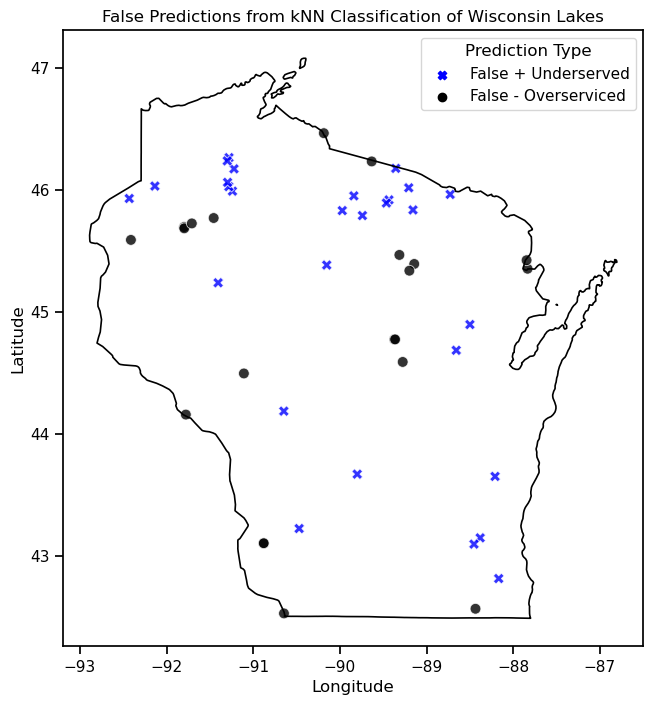
\includegraphics[keepaspectratio]{ParkSiteSelection_files/figure-pdf/fig-knn-false-predictions-output-1.png}}

}

\caption{\label{fig-knn-false-predictions}False positive and false
negative predictions from the kNN model mapped onto the state of
Wisconsin.}

\end{figure}%

The map in Figure~\ref{fig-knn-false-predictions} presents a
visualization of false predictions generated by the KNN classification
model trained to identify which Wisconsin lakes have public
services---such as boat landings, beaches, or parks---based.
Specifically, it highlights two important categories of interest for
policy consideration: underserved lakes and overserviced lakes.

\section{Further Discussion}\label{further-discussion}

Lakes marked with blue ``x'' symbols represent false positives, or
underserved lakes. These underserved lakes are those that the model
predicted to have public services, because they are similar to other
lakes that do, but that in reality do not have public services. These
lakes may warrant further investigation as candidates for the addition
of public accommodations.

Conversely, lakes marked with black dots represent false negatives, or
overserviced lakes. These overserviced lakes are those where the model
predicted no public services should be present but that are currently
are serviced with boat landings, beaches, or parks. These may be
examples of lakes whose public services might be considered for
decommission or retirement.

Both underserved and overserved lakes are widely distributed throughout
the state. This spatial analysis offers a critical bridge between
predictive modeling and those audiences who may consume this information
as they look to make and implement lake management policy. By
identifying specific lakes for which the model's prediction diverges
from current reality, this map serves as a guide for natural resource
managers, planners, and local officials for further review.

\subsection{Limitations + Weaknesses}\label{limitations-weaknesses}

Nunc ac dignissim magna. Vestibulum vitae egestas elit. Proin feugiat
leo quis ante condimentum, eu ornare mauris feugiat. Pellentesque
habitant morbi tristique senectus et netus et malesuada fames ac turpis
egestas. Mauris cursus laoreet ex, dignissim bibendum est posuere
iaculis. Suspendisse et maximus elit. In fringilla gravida ornare.
Aenean id lectus pulvinar, sagittis felis nec, rutrum risus. Nam vel
neque eu arcu blandit fringilla et in quam. Aliquam luctus est sit amet
vestibulum eleifend. Phasellus elementum sagittis molestie. Proin tempor
lorem arcu, at condimentum purus volutpat eu. Fusce et pellentesque
ligula. Pellentesque id tellus at erat luctus fringilla. Suspendisse
potenti.

Etiam maximus accumsan gravida. Maecenas at nunc dignissim, euismod enim
ac, bibendum ipsum. Maecenas vehicula velit in nisl aliquet ultricies.
Nam eget massa interdum, maximus arcu vel, pretium erat. Maecenas sit
amet tempor purus, vitae aliquet nunc. Vivamus cursus urna velit,
eleifend dictum magna laoreet ut. Duis eu erat mollis, blandit magna id,
tincidunt ipsum. Integer massa nibh, commodo eu ex vel, venenatis
efficitur ligula. Integer convallis lacus elit, maximus eleifend lacus
ornare ac. Vestibulum scelerisque viverra urna id lacinia. Vestibulum
ante ipsum primis in faucibus orci luctus et ultrices posuere cubilia
curae; Aenean eget enim at diam bibendum tincidunt eu non purus. Nullam
id magna ultrices, sodales metus viverra, tempus turpis.

Duis ornare ex ac iaculis pretium. Maecenas sagittis odio id erat
pharetra, sit amet consectetur quam sollicitudin. Vivamus pharetra quam
purus, nec sagittis risus pretium at. Nullam feugiat, turpis ac accumsan
interdum, sem tellus blandit neque, id vulputate diam quam semper nisl.
Donec sit amet enim at neque porttitor aliquet. Phasellus facilisis
nulla eget placerat eleifend. Vestibulum non egestas eros, eget lobortis
ipsum. Nulla rutrum massa eget enim aliquam, id porttitor erat luctus.
Nunc sagittis quis eros eu sagittis. Pellentesque dictum, erat at
pellentesque sollicitudin, justo augue pulvinar metus, quis rutrum est
mi nec felis. Vestibulum efficitur mi lorem, at elementum purus
tincidunt a. Aliquam finibus enim magna, vitae pellentesque erat
faucibus at. Nulla mauris tellus, imperdiet id lobortis et, dignissim
condimentum ipsum. Morbi nulla orci, varius at aliquet sed, facilisis id
tortor. Donec ut urna nisi.

\subsection{Suggestions For Further
Work}\label{suggestions-for-further-work}

Lorem ipsum dolor sit amet, consectetur adipiscing elit. Duis sagittis
posuere ligula sit amet lacinia. Duis dignissim pellentesque magna,
rhoncus congue sapien finibus mollis. Ut eu sem laoreet, vehicula ipsum
in, convallis erat. Vestibulum magna sem, blandit pulvinar augue sit
amet, auctor malesuada sapien. Nullam faucibus leo eget eros hendrerit,
non laoreet ipsum lacinia. Curabitur cursus diam elit, non tempus ante
volutpat a. Quisque hendrerit blandit purus non fringilla. Integer sit
amet elit viverra ante dapibus semper. Vestibulum viverra rutrum enim,
at luctus enim posuere eu. Orci varius natoque penatibus et magnis dis
parturient montes, nascetur ridiculus mus.

Nunc ac dignissim magna. Vestibulum vitae egestas elit. Proin feugiat
leo quis ante condimentum, eu ornare mauris feugiat. Pellentesque
habitant morbi tristique senectus et netus et malesuada fames ac turpis
egestas. Mauris cursus laoreet ex, dignissim bibendum est posuere
iaculis. Suspendisse et maximus elit. In fringilla gravida ornare.
Aenean id lectus pulvinar, sagittis felis nec, rutrum risus. Nam vel
neque eu arcu blandit fringilla et in quam. Aliquam luctus est sit amet
vestibulum eleifend. Phasellus elementum sagittis molestie. Proin tempor
lorem arcu, at condimentum purus volutpat eu. Fusce et pellentesque
ligula. Pellentesque id tellus at erat luctus fringilla. Suspendisse
potenti.

\section{Summary + Conclusions}\label{summary-conclusions}

Maecenas turpis velit, ultricies non elementum vel, luctus nec nunc.
Nulla a diam interdum, faucibus sapien viverra, finibus metus. Donec non
tortor diam. In ut elit aliquet, bibendum sem et, aliquam tortor. Donec
congue, sem at rhoncus ultrices, nunc augue cursus erat, quis porttitor
mauris libero ut ex. Nullam quis leo urna. Donec faucibus ligula eget
pellentesque interdum. Lorem ipsum dolor sit amet, consectetur
adipiscing elit. Aenean rhoncus interdum erat ut ultricies. Aenean
tempus ex non elit suscipit, quis dignissim enim efficitur. Proin
laoreet enim massa, vitae laoreet nulla mollis quis.

Vestibulum ultrices, tortor at mattis porta, odio nisi rutrum nulla, sit
amet tincidunt eros quam facilisis tellus. Fusce eleifend lectus in
elementum lacinia. Nam auctor nunc in massa ullamcorper, sit amet auctor
ante accumsan. Nam ut varius metus. Curabitur eget tristique leo. Cras
finibus euismod erat eget elementum. Integer vel placerat ex. Ut id eros
quis lectus lacinia venenatis hendrerit vel ante.

Etiam congue quam eget velit convallis, eu sagittis orci vestibulum.
Vestibulum at massa turpis. Curabitur ornare ex sed purus vulputate,
vitae porta augue rhoncus. Phasellus auctor suscipit purus, vel
ultricies nunc. Nunc eleifend nulla ac purus volutpat, id fringilla
felis aliquet. Duis vitae porttitor nibh, in rhoncus risus. Vestibulum a
est vitae est tristique vehicula. Proin mollis justo id est tempus
hendrerit. Praesent suscipit placerat congue. Aliquam eu elit gravida,
consequat augue non, ultricies sapien. Nunc ultricies viverra ante, sit
amet vehicula ante volutpat id. Etiam tempus purus vitae tellus mollis
viverra. Donec at ornare mauris. Aliquam sodales hendrerit ornare.
Suspendisse accumsan lacinia sapien, sit amet imperdiet dui molestie ut.

Etiam non efficitur urna, quis elementum nisi. Mauris posuere a augue
vel gravida. Praesent luctus erat et ex iaculis interdum. Nulla
vestibulum quam ac nunc consequat vulputate. Nullam iaculis lobortis sem
sit amet fringilla. Aliquam semper, metus ut blandit semper, nulla velit
fermentum sapien, fermentum ultrices dolor sapien sed leo. Vestibulum
molestie faucibus magna, at feugiat nulla ullamcorper a. Aliquam erat
volutpat. Praesent scelerisque magna a justo maximus, sit amet suscipit
mauris tempor. Nulla nec dolor eget ipsum pellentesque lobortis a in
ipsum. Morbi turpis turpis, fringilla a eleifend maximus, viverra nec
neque. Class aptent taciti sociosqu ad litora torquent per conubia
nostra, per inceptos himenaeos.

\section{Appendicies}\label{appendicies}

\textbf{Mapping Wisconsin's Shape and Lake Locations}

To generate the maps featured in this analysis, the shape of the state
of Wisconsin was retrieved from a public \textbf{GeoJSON} file hosted on
GitHub. GeoJSON is a geospatial data format based on JSON (JavaScript
Object Notation) that stores geographic features such as points, lines,
and polygons. In this case, the boundary polygon of Wisconsin serves as
the base layer for the map.

The file is read into a \textbf{GeoDataFrame} using the
\texttt{GeoPandas} library (\texttt{gpd}). GeoPandas is an extension of
Pandas that enables spatial operations and plotting by introducing a
\texttt{geometry} column capable of storing shapely geometries. A simple
function was written to check whether the Wisconsin GeoJSON file already
exists locally and, if not, to download and store it from a known remote
source.

Lake location data from the Wisconsin Department of Natural Resources
(WDNR) was merged with additional columns indicating the presence of
public services. Using \texttt{gpd.points\_from\_xy()}, each lake's
longitude and latitude values were converted to a point geometry, and
the data were also cast into a GeoDataFrame.

To ensure proper alignment on the map, both the Wisconsin boundary and
the lake point geometries were assigned the same \textbf{Coordinate
Reference System (CRS)}: EPSG:4326, which corresponds to the standard
WGS84 system using degrees of latitude and longitude.

\begin{itemize}
\item
  EPSG:4326 refers to a specific coordinate reference system (CRS) that
  is widely used for geographic data. It is part of a registry
  maintained by the European Petroleum Survey Group (EPSG), which
  assigns numeric codes to standard spatial reference systems. EPSG:4326
  specifies that coordinates are expressed in degrees of latitude and
  longitude, based on the WGS84 datum.
\item
  WGS84, or the World Geodetic System 1984, is a global reference system
  used by GPS and many mapping applications. It defines the shape of the
  Earth as an ellipsoid and provides a consistent framework for locating
  points on the Earth's surface. When spatial data is aligned to WGS84,
  it can be accurately mapped and compared across different datasets and
  tools, making it a common default in global mapping applications and
  open geospatial data formats.
\end{itemize}

Plotting was accomplished using \textbf{Matplotlib} and
\textbf{Seaborn}, with lake points styled according to the presence or
absence of public services (e.g., boat landings, beaches, or parks).
This overlay provides a spatial perspective that supports both
exploratory analysis and the interpretation of model predictions.

\section{Scratch Space}\label{scratch-space}

\section{Outtakes}\label{outtakes}

This paper demonstrates a data science process that doesn't require a
continually updated model. Unlike situations where data changes
frequently (e.g., online shopping recommendations), the number of lakes
in Wisconsin is relatively static. Our goal is to provide a one-time
analysis identifying potential discrepancies between existing public
services and lake needs. This information will be valuable for policy
discussions across various government levels, where a single,
well-documented analysis is more suitable than a dynamic model.

Moreover, according to Srinivas et al. (2022) domain knowledge plays a
critical role in feature engineering, a key step in the data science
pipeline. Srinivas et al.~argue that while automation can assist in
expanding the feature space, it cannot replace the human ability to
apply domain-specific knowledge to identify meaningful features. This
sentiment is echoed in the work of M. A. Waller and Fawcett (2013) who
assert that the intersection of data science with specific domains
necessitates a deep understanding of both the data and contexts in which
it is applied. Without this understanding, data scientists may struggle
to derive insights that are both relevant and useful.

``Overfitting is a common problem in machine learning, where a model
performs well on training data but does not genrealize well to unseen
datas (test data). If a model suffers from overfitting, we also say that
the model has a high variance, which can be caused by having too many
parameters, leading to a model that is too complex given the underlying
data.'' (Raschka and Mirjalili 2019, p 75)

\begin{Shaded}
\begin{Highlighting}[]
\NormalTok{log\_pairplot }\OperatorTok{=}\NormalTok{ sns.pairplot(}
\NormalTok{    df[[}\StringTok{\textquotesingle{}size\textquotesingle{}}\NormalTok{,}\StringTok{\textquotesingle{}maxdepth\textquotesingle{}}\NormalTok{,}\StringTok{\textquotesingle{}meandepth\textquotesingle{}}\NormalTok{,}\StringTok{\textquotesingle{}hasservice\textquotesingle{}}\NormalTok{]],}
\NormalTok{    hue}\OperatorTok{=}\StringTok{\textquotesingle{}hasservice\textquotesingle{}}\NormalTok{, aspect}\OperatorTok{=}\DecValTok{2}\NormalTok{)}

\ControlFlowTok{for}\NormalTok{ ax }\KeywordTok{in}\NormalTok{ log\_pairplot.axes.flatten():  }\CommentTok{\# Iterate over all subplots}
\NormalTok{    ax.set\_xscale(}\StringTok{\textquotesingle{}log\textquotesingle{}}\NormalTok{)}
\NormalTok{    ax.set\_yscale(}\StringTok{\textquotesingle{}log\textquotesingle{}}\NormalTok{)}
\end{Highlighting}
\end{Shaded}

\begin{figure}[H]

\centering{

\pandocbounded{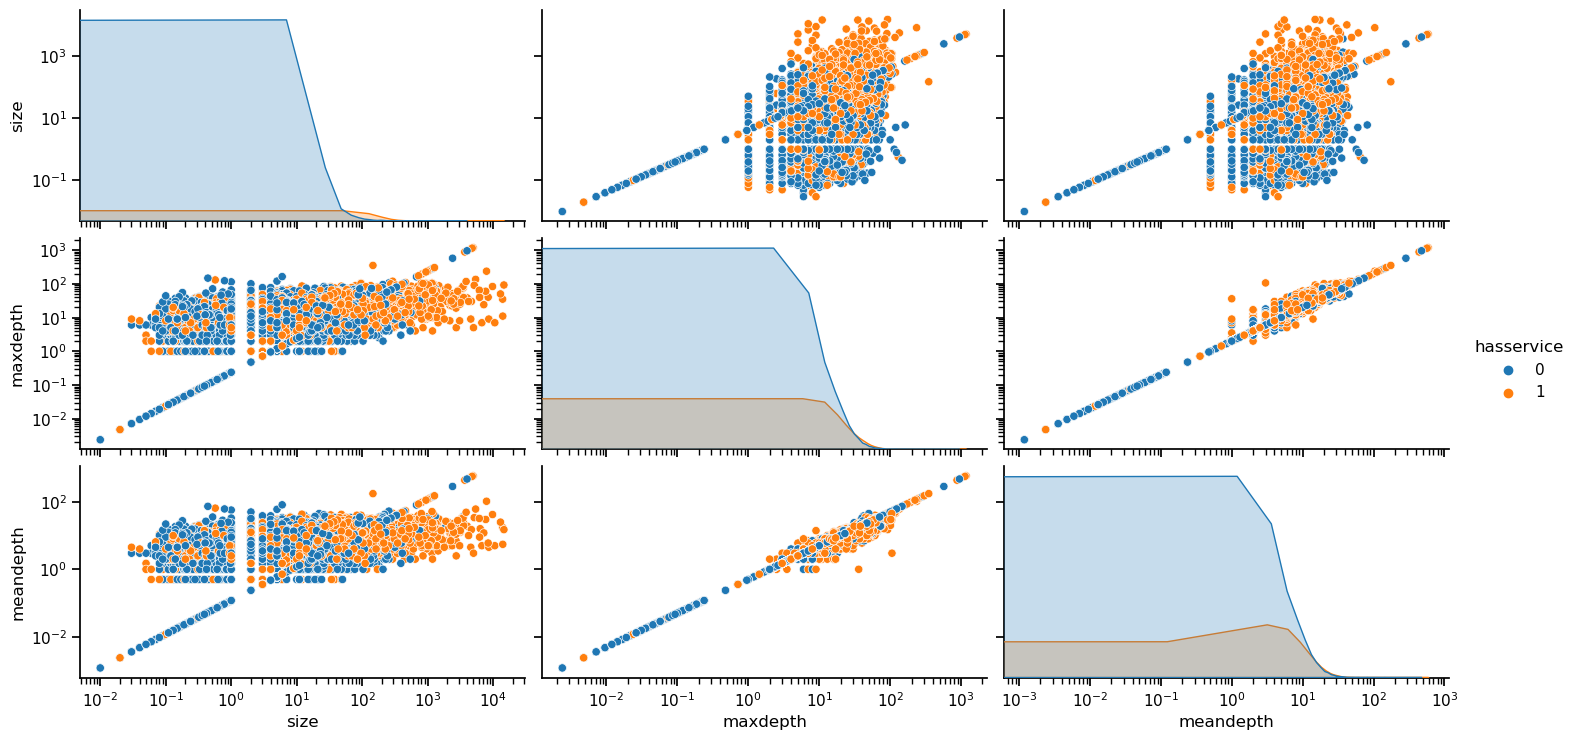
\includegraphics[keepaspectratio]{ParkSiteSelection_files/figure-pdf/fig-logpairplot_2-output-1.png}}

}

\caption{\label{fig-logpairplot_2}A Traditional Pairplot.}

\end{figure}%

\section*{References}\label{references}
\addcontentsline{toc}{section}{References}

\phantomsection\label{refs}
\begin{CSLReferences}{1}{0}
\bibitem[\citeproctext]{ref-bendor2013modeling}
BenDor, Todd, James Westervelt, Yan Song, and Jared O. Sexton. 2013.
{``Modeling Park Development Through Regional Land Use Change
Simulation.''} \emph{Land Use Policy} 30 (1): 1--12.
\url{https://doi.org/10.1016/j.landusepol.2012.02.001}.

\bibitem[\citeproctext]{ref-Breiman2001culture}
Breiman, Leo. 2001. {``Statistical Modeling: The Two Cultures.''}
\emph{Statistical Science} 16 (3): 199--215.
\url{http://www.jstor.org/stable/2676681}.

\bibitem[\citeproctext]{ref-carvalho2024new}
Carvalho, J. C. S., T. C. Pimenta, A. C. P. Silverio, M. A. Carvalho,
and J. P. C. S. Carvalho. 2024. {``A New Data Science Model with
Supervised Learning and Its Application on Pesticide Poisoning Diagnosis
in Rural Workers.''} \emph{IEEE Access} 12: 40871--82.
\url{https://doi.org/10.1109/access.2024.3375764}.

\bibitem[\citeproctext]{ref-Chief2014Engaging}
Chief, K., A. M. Meadow, and K. P. Whyte. 2016. {``Engaging Southwestern
Tribes in Sustainable Water Resources Topics and Management.''}
\emph{Water} 8: 350. \url{https://doi.org/10.3390/w8080350}.

\bibitem[\citeproctext]{ref-Elbakidz2021hetero}
Elbakidze, L., and Q. Beeson. 2021. {``State Regulatory Heterogeneity
and Compliance with the Clean Water and Safe Drinking Water Acts.''}
\emph{Water Resources Research} 57.
\url{https://doi.org/10.1029/2020wr028952}.

\bibitem[\citeproctext]{ref-garn2003why}
Garn, Herbert S., John F. Elder, and Dale M. Robertson. 2003. \emph{Why
Study Lakes?: An Overview of USGS Lake Studies in Wisconsin}. Reston,
Virginia: U.S. Geological Survey.

\bibitem[\citeproctext]{ref-gutman2021becoming}
Gutman, Alex J, and Jordan Goldmeier. 2021. \emph{Becoming a Data Head:
How to Think, Speak, and Understand Data Science, Statistics, and
Machine Learning}. John Wiley \& Sons.

\bibitem[\citeproctext]{ref-james2023introduction}
James, Gareth, Daniela Witten, Trevor Hastie, Robert Tibshirani, and
Jonathan Taylor. 2023. \emph{An Introduction to Statistical Learning:
With Applications in Python}. 2023rd ed. Cham, Switzerland: Springer.

\bibitem[\citeproctext]{ref-kretschmann2011citizen}
Kretschmann, A., A. Drum, N. L. D. Center, and M. Waters. 2011. {``A
Citizen Science Program for Monitoring Lake Stages in Northern
Wisconsin.''} In \emph{AGU Fall Meeting Abstracts}, 2011:ED23C--0641.

\bibitem[\citeproctext]{ref-lillie1983limnological}
Lillie, Richard A., and James W. Mason. 1983. {``Limnological
Characteristics of Wisconsin Lakes.''} Technical Bulletin 138. Madison,
Wisconsin: Wisconsin Department of Natural Resources.

\bibitem[\citeproctext]{ref-Martins2021earlyprediction}
Martins, M. V., D. Tolledo, J. Machado, L. M. Baptista, and V. Realinho.
2021. {``Early Prediction of Student's Performance in Higher Education:
A Case Study.''} In \emph{Trends and Applications in Information Systems
and Technologies: Volume 1 9}, 166--75. Springer International
Publishing.

\bibitem[\citeproctext]{ref-wisconsin_dnr_lake_modeling_suite}
Natural Resources Lake Modeling, Wisconsin Department of. n.d. {``Lake
Modeling Suite.''} \url{https://dnr.wisconsin.gov/topic/Lakes/Model}.

\bibitem[\citeproctext]{ref-wisconsin_dnr_swims}
Natural Resources SWIMS Pages, Wisconsin Department of. n.d. {``Surface
Water Integrated Monitoring System (SWIMS).''}
\url{https://dnr.wisconsin.gov/topic/SurfaceWater/SWIMS}.

\bibitem[\citeproctext]{ref-nelson2023confident}
Nelson, Adam Ross. 2023. \emph{Confident Data Science: Discover the
Essential Skills of Data Science}. 1st ed. London: Kogan Page.

\bibitem[\citeproctext]{ref-raschka2019python}
Raschka, Sebastian, and Vahid Mirjalili. 2019. \emph{Python Machine
Learning: Machine Learning and Deep Learning with Python, Scikit-Learn,
and TensorFlow 2}. 3rd ed. Birmingham, UK: Packt Publishing.

\bibitem[\citeproctext]{ref-scikit-learn-cross-validation2023}
Scikit-Learn. 2023. {``Cross-Validation: Choosing the Best Model.''}
\url{https://scikit-learn.org/stable/modules/cross_validation.html\#cross-validation}.

\bibitem[\citeproctext]{ref-Spear2020Application}
Spear, M. J., H. S. Embke, P. J. Krysan, and M. J. V. Zanden. 2020.
{``Application of Edna as a Tool for Assessing Fish Population
Abundance.''} \emph{Environmental DNA} 3: 83--91.
\url{https://doi.org/10.1002/edn3.94}.

\bibitem[\citeproctext]{ref-Srinivas2022feature}
Srinivas, K., T. Tateishi, D. K. I. Weidele, U. Khurana, H. Samulowitz,
T. Takahashi, D. Wang, and L. Amini. 2022. {``Semantic Feature Discovery
with Code Mining and Semantic Type Detection.''} \emph{Proceedings of
the AAAI Conference on Artificial Intelligence} 36: 13224--26.
\url{https://doi.org/10.1609/aaai.v36i11.21735}.

\bibitem[\citeproctext]{ref-Thornton2013Stakeholder}
Thornton, J. A. 2013. {``Stakeholder Participation in Lake Management in
Wisconsin (Usa).''} \emph{Lakes \&Amp; Reservoirs: Science, Policy and
Management for Sustainable Use} 18: 27--33.
\url{https://doi.org/10.1111/lre.12013}.

\bibitem[\citeproctext]{ref-Waller2018Ecology}
Waller, D. M., and N. J. Reo. 2018. {``First Stewards: Ecological
Outcomes of Forest and Wildlife Stewardship by Indigenous Peoples of
Wisconsin, Usa.''} \emph{Ecology and Society} 23.
\url{https://doi.org/10.5751/es-09865-230145}.

\bibitem[\citeproctext]{ref-Waller2013bigdata}
Waller, M. A., and S. E. Fawcett. 2013. {``Data Science, Predictive
Analytics, and Big Data: A Revolution That Will Transform Supply Chain
Design and Management.''} \emph{Journal of Business Logistics} 34:
77--84. \url{https://doi.org/10.1111/jbl.12010}.

\bibitem[\citeproctext]{ref-wisconsin_dnr_lake_pages}
Wisconsin Department of Natural Resources. 2024. {``Wisconsin Department
of Natural Resources Lake Pages.''}
\url{https://apps.dnr.wi.gov/lakes/lakepages/Results.aspx?advanced=true&wbic=}.

\end{CSLReferences}




\end{document}
